\documentclass[a4paper,12pt]{article}
\usepackage[T1,T2A]{fontenc}
\usepackage[utf8]{inputenc}
\usepackage[english,russian]{babel}
\usepackage{amsmath,amsfonts,amssymb}
\usepackage{graphicx}
\usepackage{pdflscape} % Для альбомных страниц
\usepackage{booktabs}
\usepackage{geometry}
\usepackage{caption}
\usepackage{afterpage}
\geometry{left=20mm, right=20mm, top=20mm, bottom=20mm}

\title{Отчёт по экзаменационной работе ДГСП}
\author{Торбин Николай}
\date{}

\begin{document}

\maketitle

\section{Теоретическая часть}
\subsection{Неформальное описание исследуемой системы}
В статье Bio1 исследуется белок STAT5 и взаимодействие его разичных форм. При помощи нескольких методов фильтрации предлагается оценивать параметры химической реакции и прогнозировать концентрации веществ. Было показано, что при данном подходе удаётся точно описывать биохимические процессы.

\subsection{Постановка задачи}
Рассмотрим следующую систему в дискретном времени
\begin{gather}\label{sys0}
    \left\{
    \begin{aligned}
        & x_1(k+1) = \theta_1 x_1(k) + x_1(k) x_2(k) + 0.1 + \alpha v_1(k),\\
        & x_2(k+1) = \theta_2 x_2(k) - x_1(k) x_2(k) + 0.1 + \alpha v_2(k),\\
        & y_1(k) = x_1(k) + \alpha w_1(k), \\
        & y_2(k) = x_2(k) + \alpha w_2(k),
    \end{aligned}
    \right.
\end{gather}
$k = 1, \dots, 800$. Здесь $(x_1, x_2)$ -- скрытое состояние, $(\theta_1, \theta_2)$ -- неизвестные параметры, $(y_1, y_2)$ -- наблюдения. $\alpha = 0.001$, $v_1, v_2, w_1, w_2$ -- шумы с нулевым средним, имеющие дискретные распределения
\begin{gather*}
    \mathbf{P}(v_1(k) = -1) = 0.6,\,  \mathbf{P}(v_1(k) = 0.2) = 0.2,\, \mathbf{P}(v_1(k) = 3) = 0.2,\\
    \mathbf{P}(v_2(k) = -1) = 0.8,\, \mathbf{P}(v_2(k) = 4) = 0.2,\\
    \mathbf{P}(w_1(k) = -7) = 0.3,\, \mathbf{P}(w_1(k) = 3) = 0.7,\\
    \mathbf{P}(w_2(k) = 7) = 0.3,\, \mathbf{P}(w_2(k) = -3) = 0.7.
\end{gather*}

В оригинальной работе Bio1 анализ системы проводился с использованием единственной наблюдаемой величины $y_2$. Для повышения точности восстановления скрытых состояний и оценки параметров в рассмотрение введена величина $y_1$, это позволило значительно улучшить результаты. 

Для одновременного оценивания параметров и состояния системы, рассмотрим расширенную систему $X(k) = (x_1, x_2, \theta_1, \theta_2)^\top$.

Тогда (\ref{sys0}) принимает вид:
\begin{gather}\label{sys}
    \left\{
    \begin{aligned}
        &X_k = a(X_{k-1}) + v_k,\\
        &y_k = A(X_k) + w_k,
    \end{aligned}
    \right.
\end{gather}
$v(k) = (v_1(k), v_2(k), 0, 0)$, $w(k) = (w_1(k), w_2(k))$.

\begin{gather*}
    a(x_1, x_2, \theta_1, \theta_2) = 
    \begin{pmatrix}
        \theta_1 x_1 + x_1 x_2 + 0.1\\ 
        \theta_2 x_2 - x_1 x_2 + 0.1\\
        \theta_1\\
        \theta_2
    \end{pmatrix},\quad A(x_1, x_2, \theta_1, \theta_2) = 
    \begin{pmatrix}
        x_1\\
        x_2
    \end{pmatrix}.
\end{gather*}

Итак, задача состоит в оценивании скрытого состояния $X_k$ по наблюдениям $y_k$.

\subsection{Методы}
Использовались следующие алгоритмы:
\begin{enumerate}
    \item Расширенный фильтр Калмана 2 порядка (EKF2),
    \item Корневая модификация EKF2 (SREKF2),
    \item Бутстреп фильтр.
\end{enumerate}

\subsubsection{Производные для EKF2}
Градиенты:
\begin{gather*}
    \nabla a(x_1, x_2, \theta_1, \theta_2) = 
        \begin{pmatrix}
            \theta_1 + x_2 & x_1 & x_1 & 0 \\
            -x_2 &\theta_2 - x_1 & 0 & x_2 \\
            0 & 0 & 1 & 0 \\
            0 & 0 & 0 & 1 
        \end{pmatrix}, \quad 
    \nabla A(x_1, x_2, \theta_1, \theta_2) = 
    \begin{pmatrix}
        1 & 0 & 0 & 0\\
        0 & 1 & 0 & 0
    \end{pmatrix}
\end{gather*}
Гессианы:
\begin{gather*}
    \nabla^2 a^1(x_1, x_2, \theta_1, \theta_2) = 
        \begin{pmatrix}
            0 &  1 & 1 & 0 \\
            1 &  0 & 0 & 0 \\
            1 &  0 & 0 & 0 \\
            0 &  0 & 0 & 0 
        \end{pmatrix}, \quad
    \nabla^2 a^2(x_1, x_2, \theta_1, \theta_2) = 
        \begin{pmatrix}
             0 & -1 & 0 & 0\\
            -1 &  0 & 0 & 1\\
             0 &  0 & 0 & 0 \\
             0 &  1 & 0 & 0 
        \end{pmatrix}, \\
    \nabla^2 a^3(x_1, x_2, \theta_1, \theta_2) = \nabla^2 a^4(x_1, x_2, \theta_1, \theta_2) =
        \begin{pmatrix}
             0 & 0 & 0 & 0 \\
             0 & 0 & 0 & 0 \\
             0 & 0 & 0 & 0 \\
             0 & 0 & 0 & 0 
        \end{pmatrix}.
\end{gather*}

\begin{gather*}
    \nabla^2 A^i(x_1, x_2, \theta_1, \theta_2) = \begin{pmatrix}
             0 & 0 & 0 & 0 \\
             0 & 0 & 0 & 0 \\
             0 & 0 & 0 & 0 \\
             0 & 0 & 0 & 0 
        \end{pmatrix},\, i = 1, 2.
\end{gather*}

\subsubsection{Параметры PF boot}
Размер пучка траекторий $N = 10000$.

Для того чтобы фильтр "находил" неизвестные параметры $(\theta_1, \theta_2)$, используется случайная инициализация, а также добавление шума к значениям параметров (с малой дисперсией). То есть моделируется пучок процессов следующего вида:
\begin{align*}
    X_k = a(X_{k-1}) + \tilde{v}(k),
\end{align*}
$\tilde{v}(k) = (\tilde{v}_1(k), \tilde{v}_2(k), \tilde{v}_3(k), \tilde{v}_4(k))^\top$,
где $\tilde{v}_1$ и $\tilde{v}_2$ имеют такое же распределение как и в реальной системе \ref{sys}, а 
\begin{gather*}
    \tilde{v}_3(k), \tilde{v}_4(k) \sim \mathcal{N}(0, (0.7)^k10^{-2})
\end{gather*}

Чтобы сохранить устойчивость системы, параметр стандартного отклонения шума выбран убывающим, то есть $\tilde{v}(k) \to v(k),\, k \to \infty$ по распределению.

Для условная плотность $p(y|X)$, используемая для пересчёта весов, аппроксимируется смесью гауссовских плотностей со модами в точках носителя $w(k)$:
\begin{multline*}
    \overline{p}(y_1, y_2|x) = \left[ 0.7 \rho(y_1, x_1-7\alpha, 10^{-3}) + 0.3 \rho(y_1, x_1+3\alpha, 10^{-3}) \right] \times \\
    \times \left[ 0.3 \rho(y_2, x_2+7\alpha, 10^{-3}) + 0.7 \rho(y_1, x_2-3\alpha, 10^{-3}) \right],
\end{multline*}
где $\rho(\cdot, \mu, \sigma)$ -- плотность $\mathcal{N}(\mu, \sigma)$.

\section{Расчетная часть}

\subsection{Параметры}

\begin{table}
    \centering
    \begin{tabular}{c|c}
        $\alpha$ & 0.01 \\
        $\theta_1$ & 0.8 \\
        $\theta_2$ & 1.5 \\
        $x_1(0)$ & 1.35 \\
        $x_2(0)$ & 0.11
    \end{tabular}
    \caption{Параметры системы}
    \label{tab:params}
\end{table}

Начальные матрицы ковариации для фильтров:
\begin{gather*}
    R_0^{PF} = \mathrm{diag}(10^{-2}, 10^{-2}, 1, 1),\quad R_0^{EKF2} = R_0^{SREKF2} = \mathrm{diag}(0, 0, 10^{-4}, 10^{-4})
\end{gather*}

Количество частиц для бутстреп фильтра $N_{PF} = 10000$. Пучок для оценки СКО методом Монте-Карло $N_{MC} = 10000$.

\subsection{Оценки состояния для одной траектории}
Далее приведены оценки фильтрации одной траектории.

\begin{landscape}
\begin{figure}[p]
\centering
\caption{Оценки $x_1$}
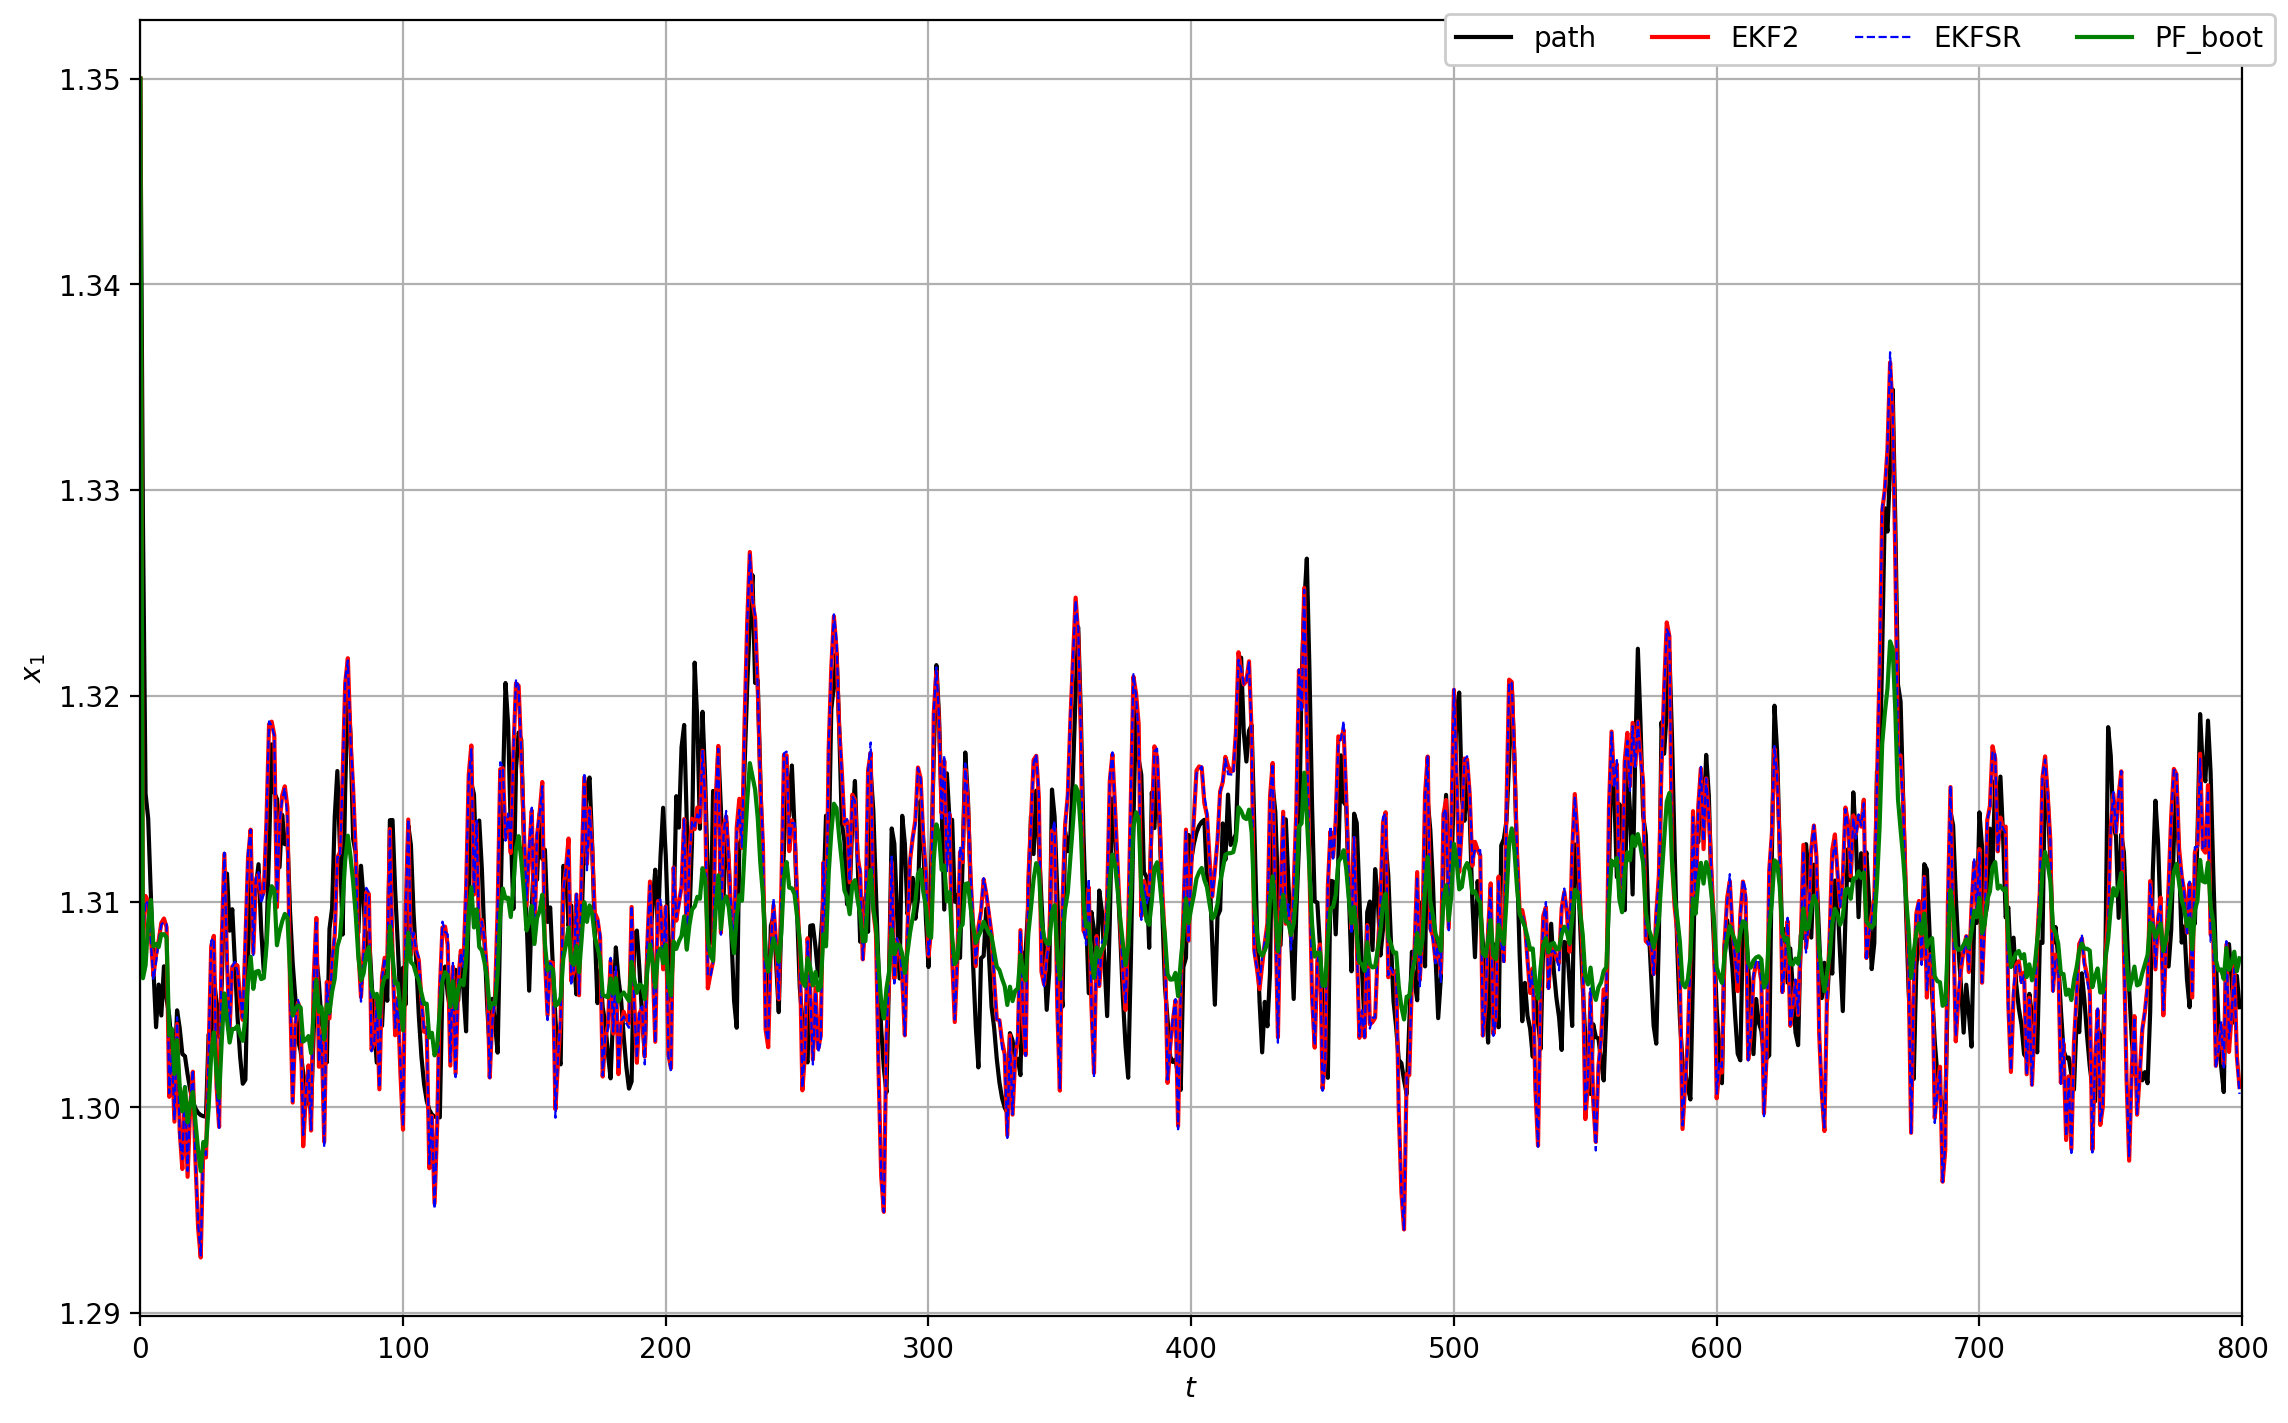
\includegraphics[width=0.95\linewidth]{x1.png}
\label{fig:x1}
\end{figure}

\begin{figure}[p]
\centering
\caption{Оценки $x_2$}
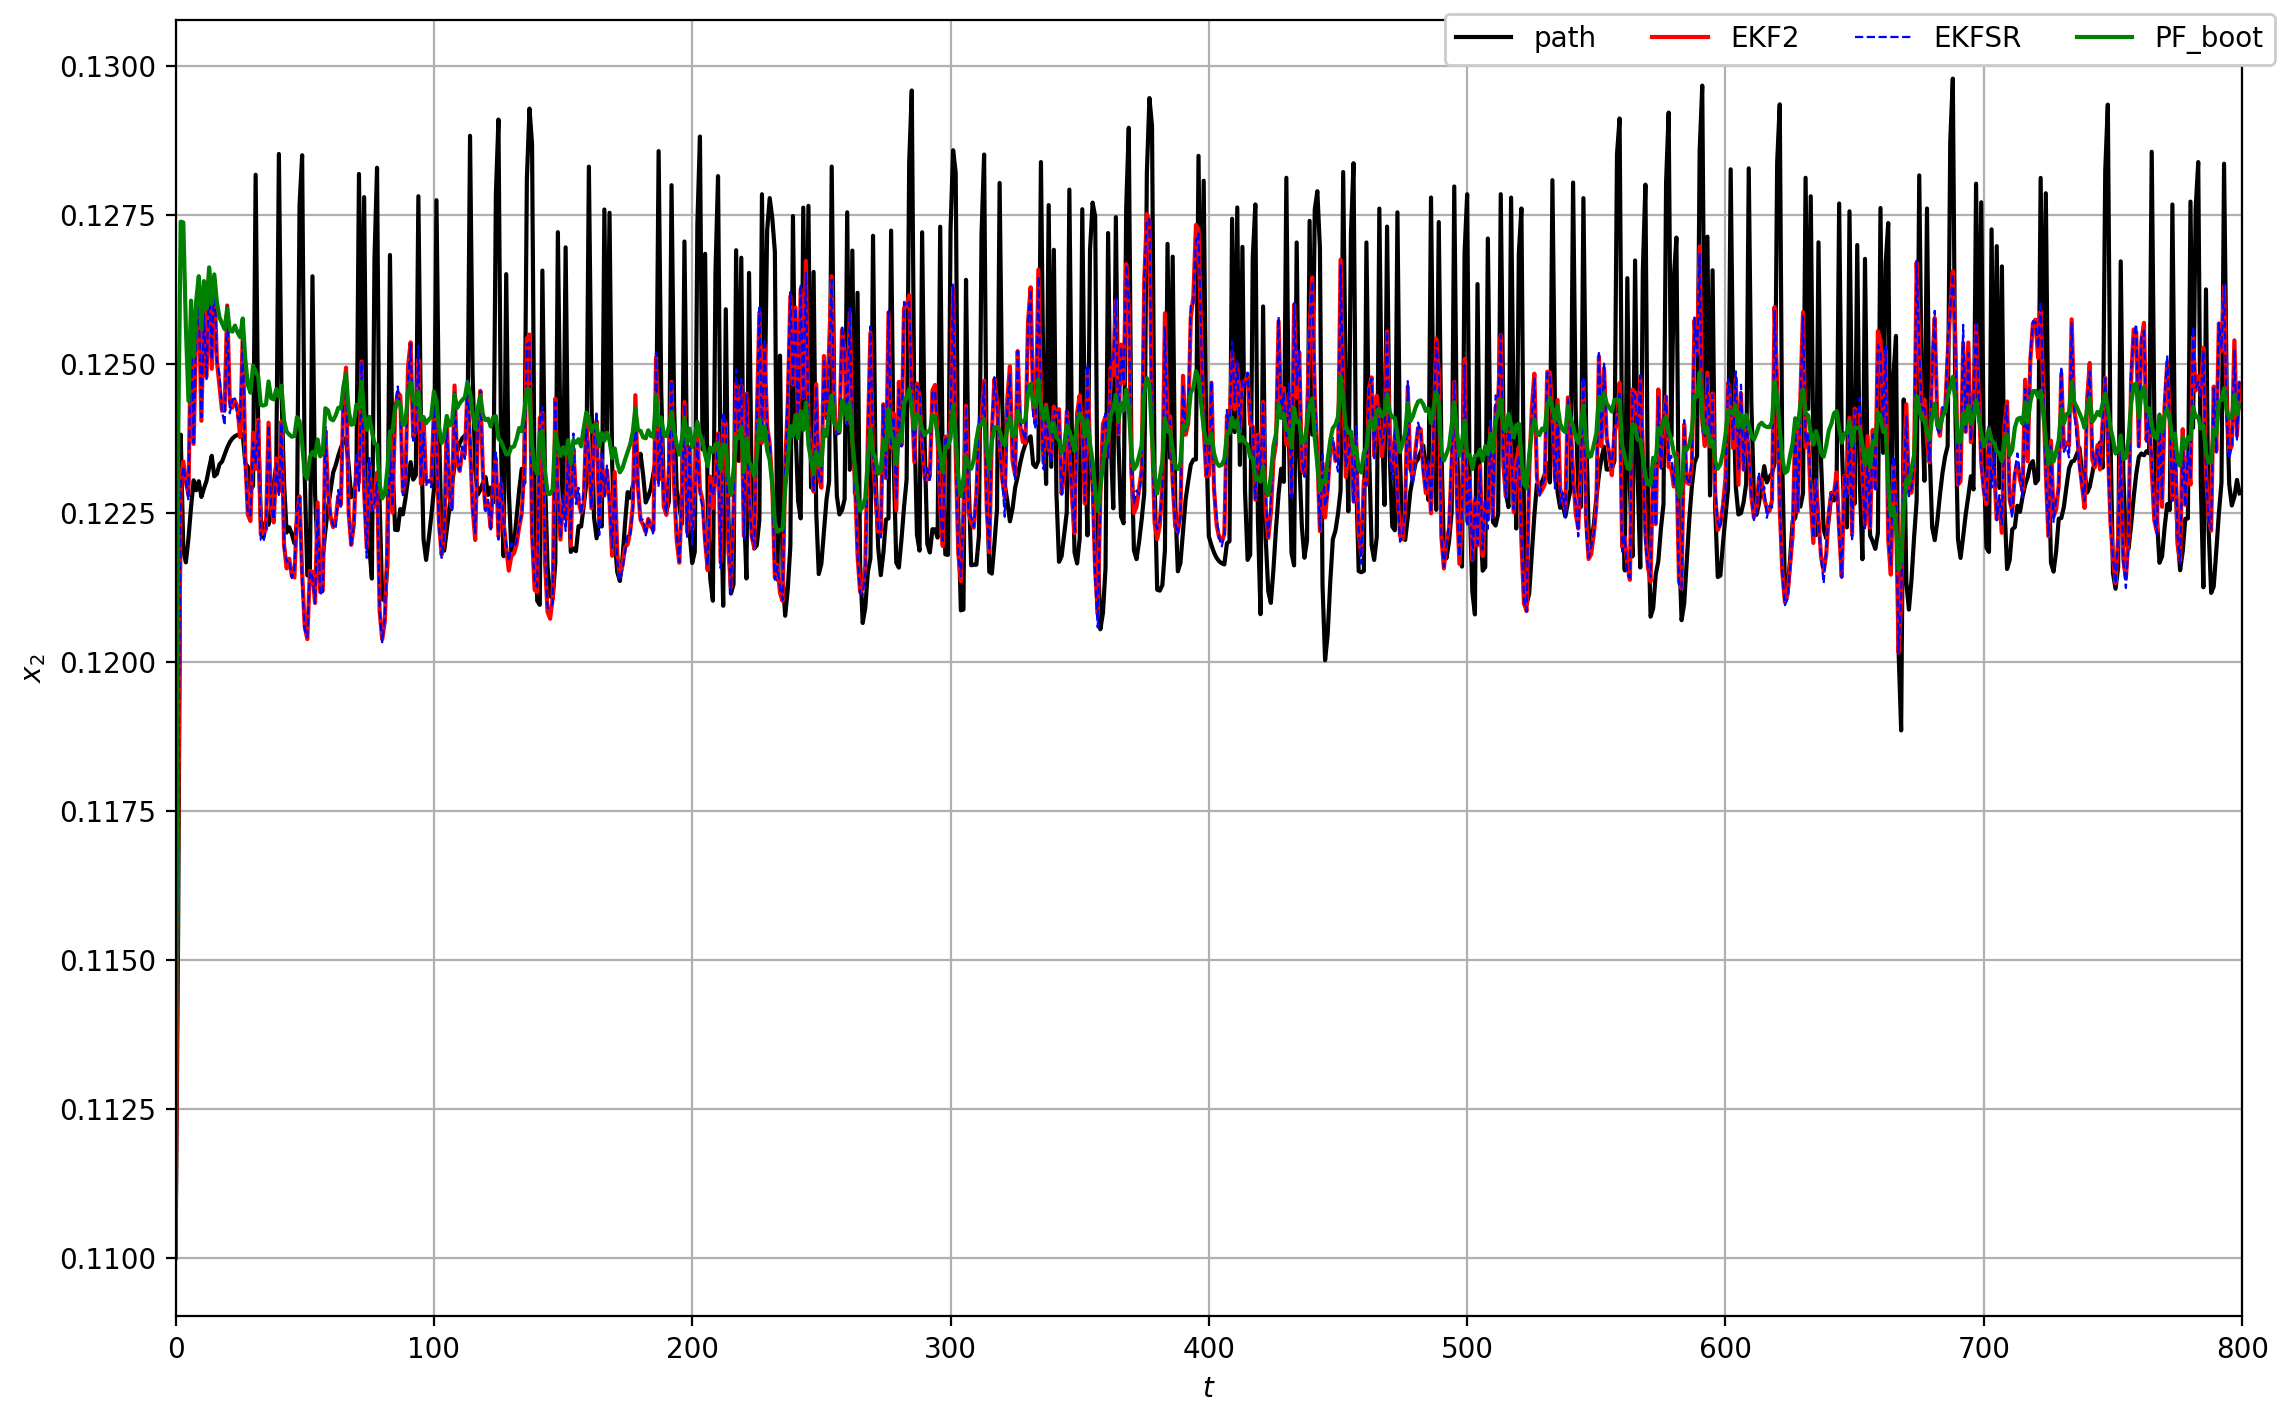
\includegraphics[width=0.95\linewidth]{x2.png}
\label{fig:x2}
\end{figure}
\end{landscape}
\begin{landscape}
\begin{figure}[p]
\centering
\caption{Оценки $\theta_1$}
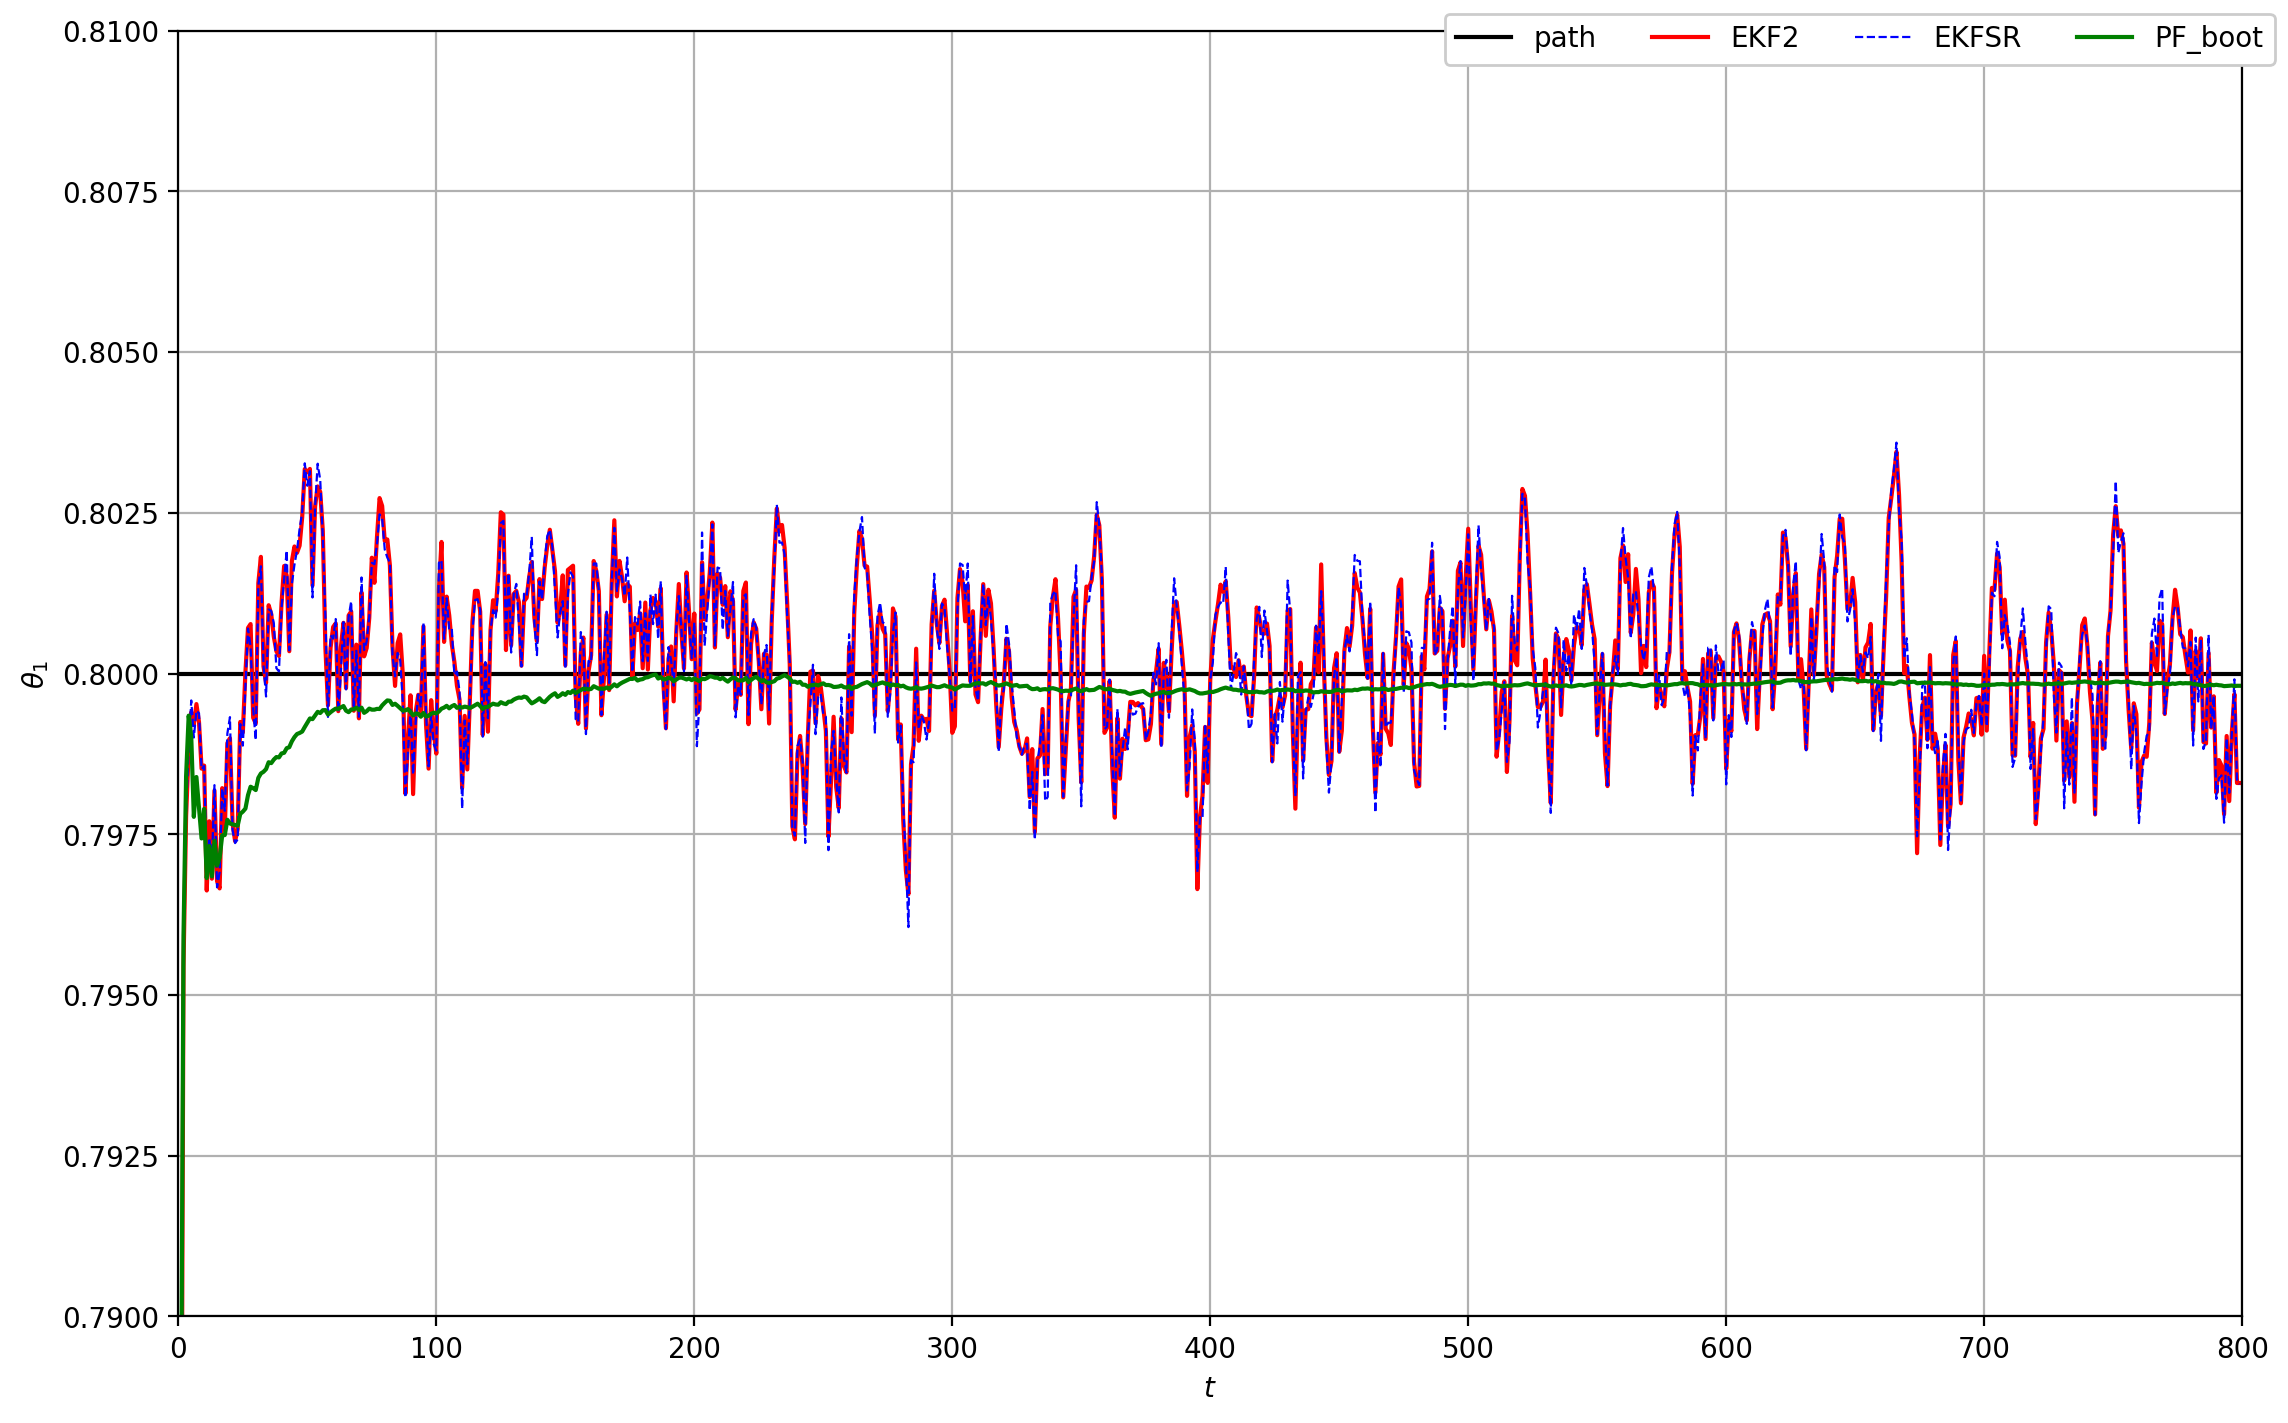
\includegraphics[width=0.95\linewidth]{theta1.png}
\label{theta1}
\end{figure}

\begin{figure}[p]
\centering
\caption{Оценки $\theta_2$}
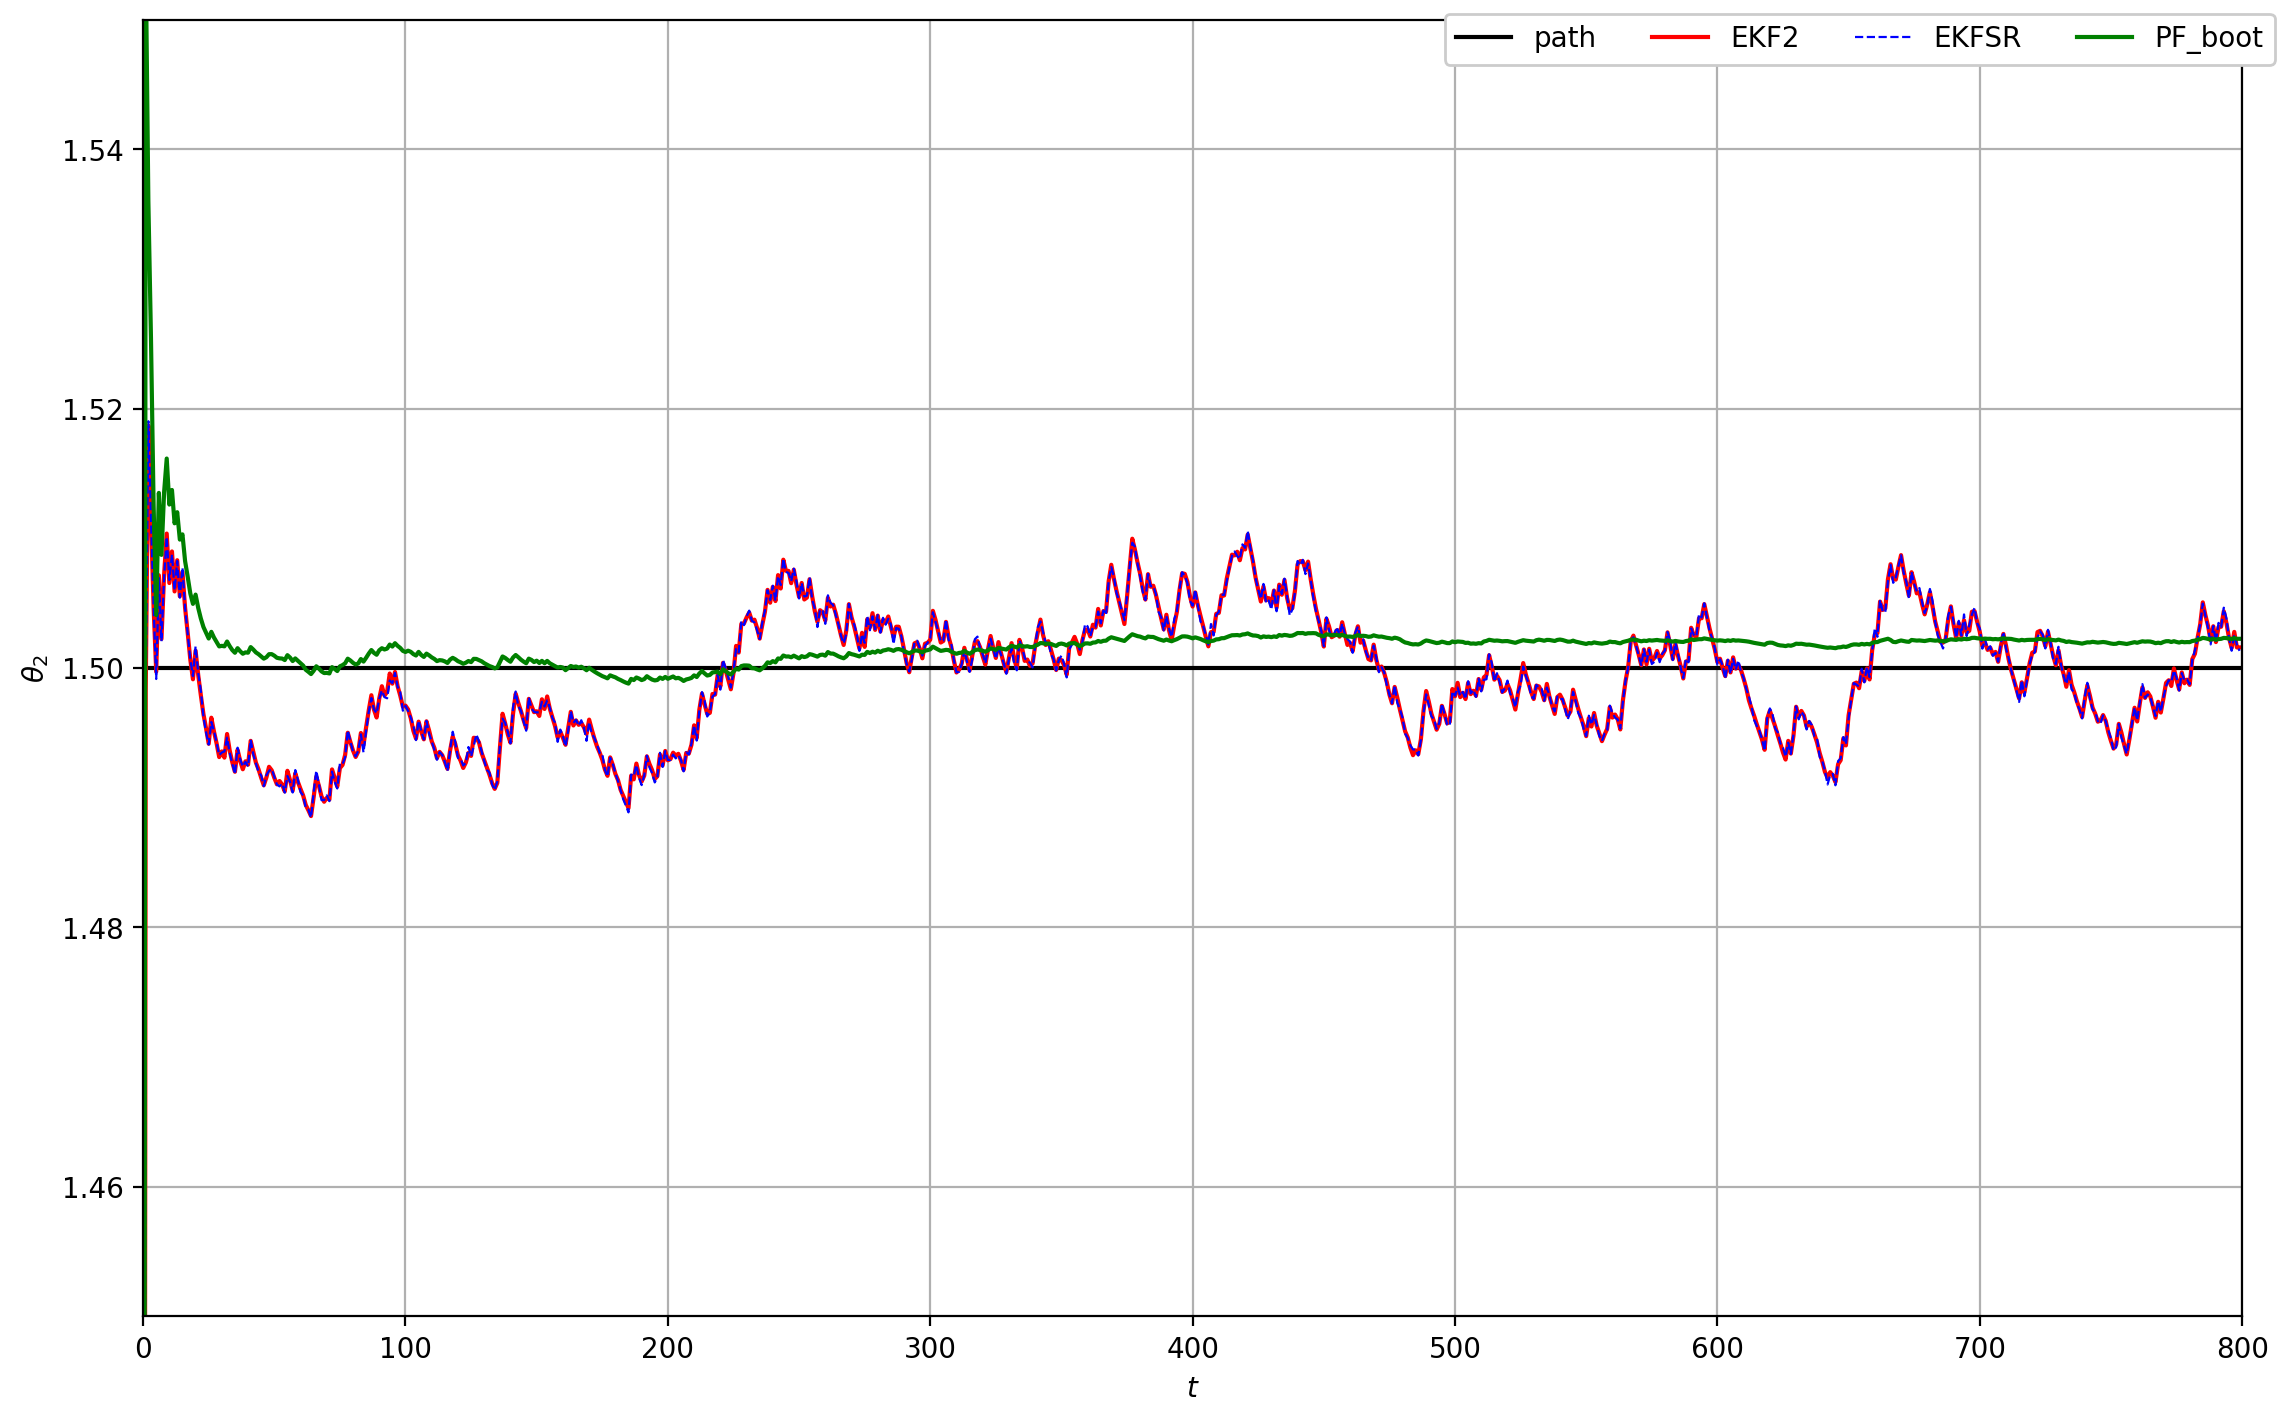
\includegraphics[width=0.95\linewidth]{theta2.png}

\label{fig:theta2}
\end{figure}
\end{landscape}

\subsection{Ошибки оценивания}
Ниже представлены графики ошибок оценивания состояния системы и параметров.

\begin{landscape}
\begin{figure}[p]
\centering
\caption{EKF2 $\pm 3\sigma(x_1)$}
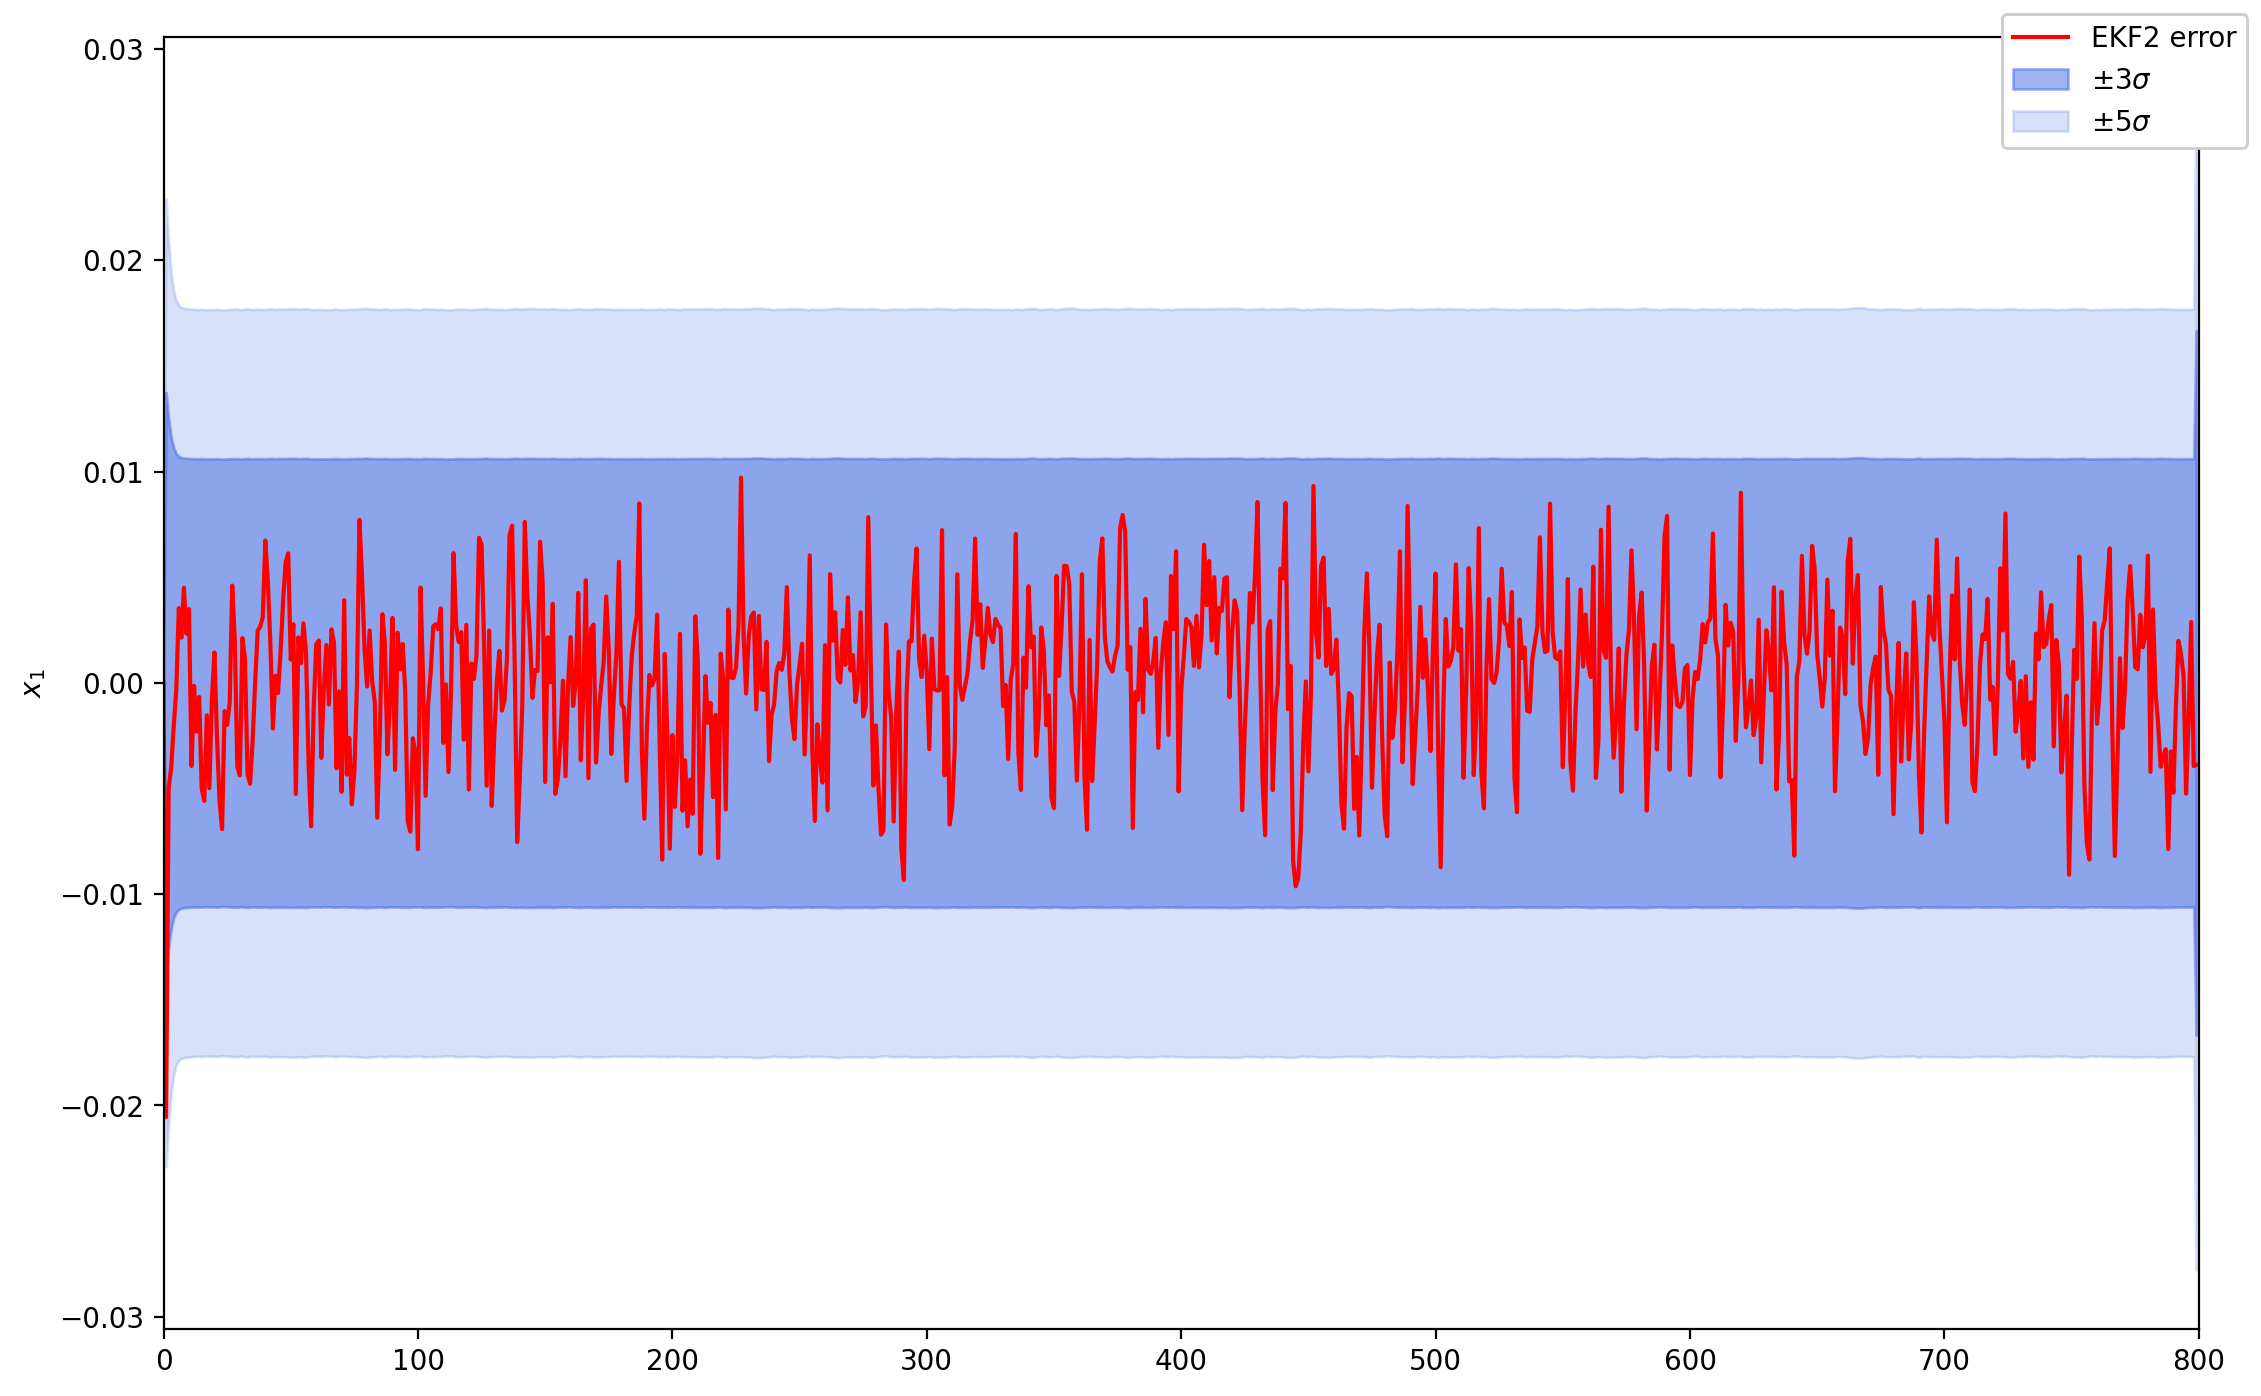
\includegraphics[width=0.95\linewidth]{EKF2_err_x1.png}
\label{fig:x1_ci}
\end{figure}

\begin{figure}[p]
\centering
\caption{EKF2 $\pm 3\sigma(x_2)$}
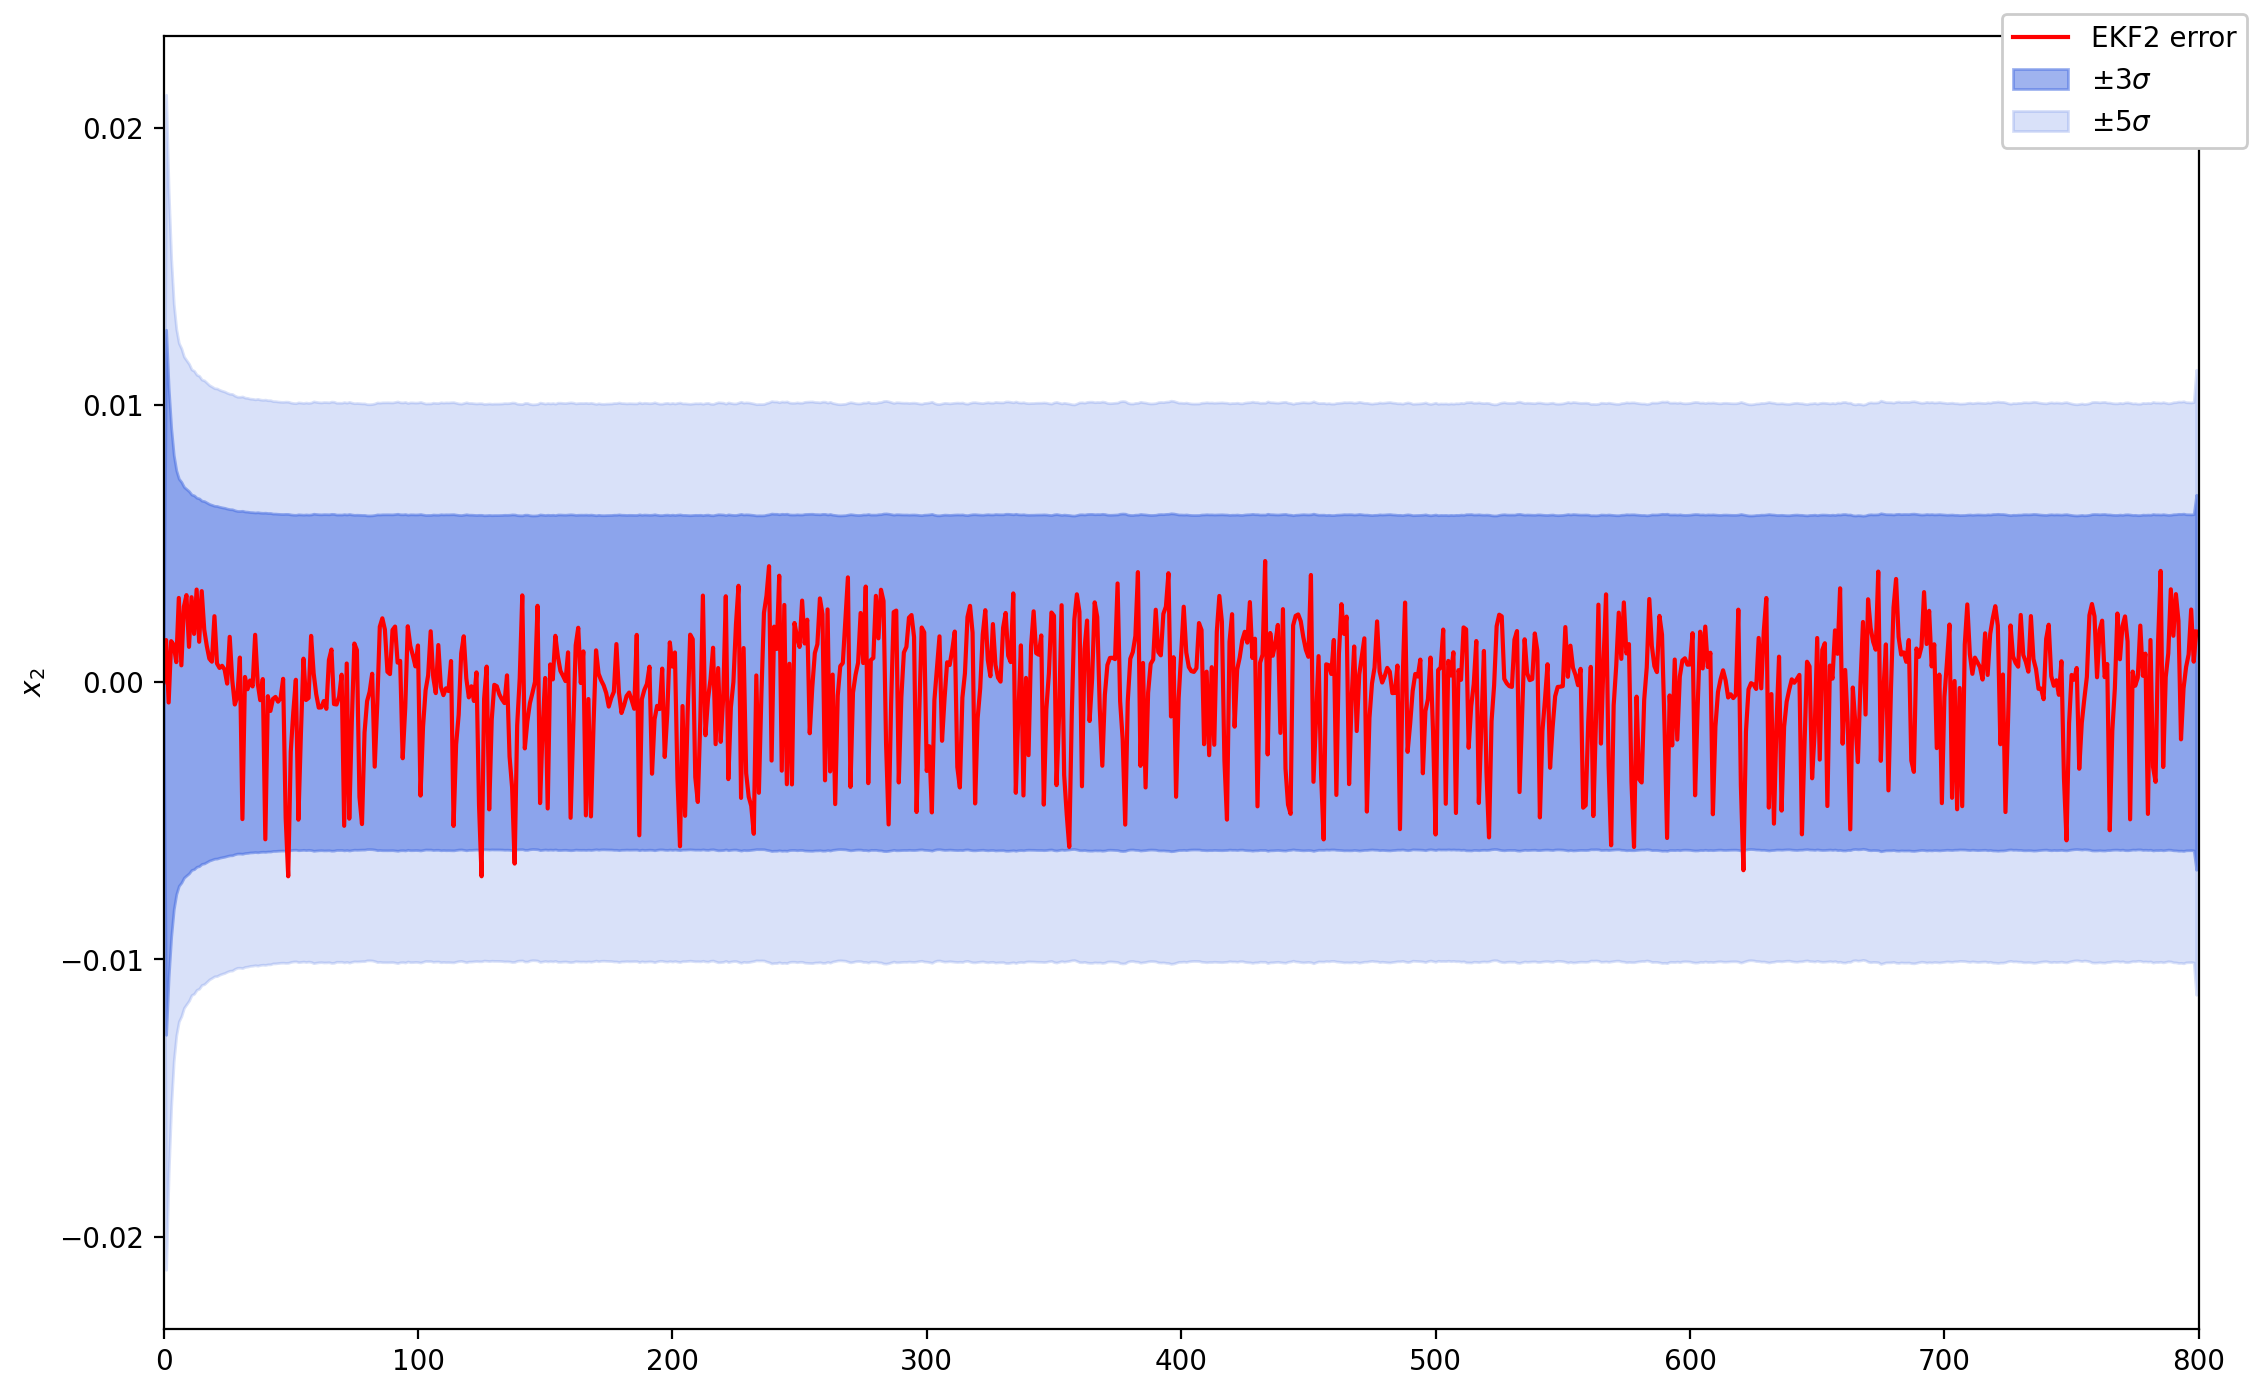
\includegraphics[width=0.95\linewidth]{EKF2_err_x2.png}
\end{figure}

\begin{figure}[p]
\centering
\caption{EKF2 $\pm 3\sigma(\theta_1)$}
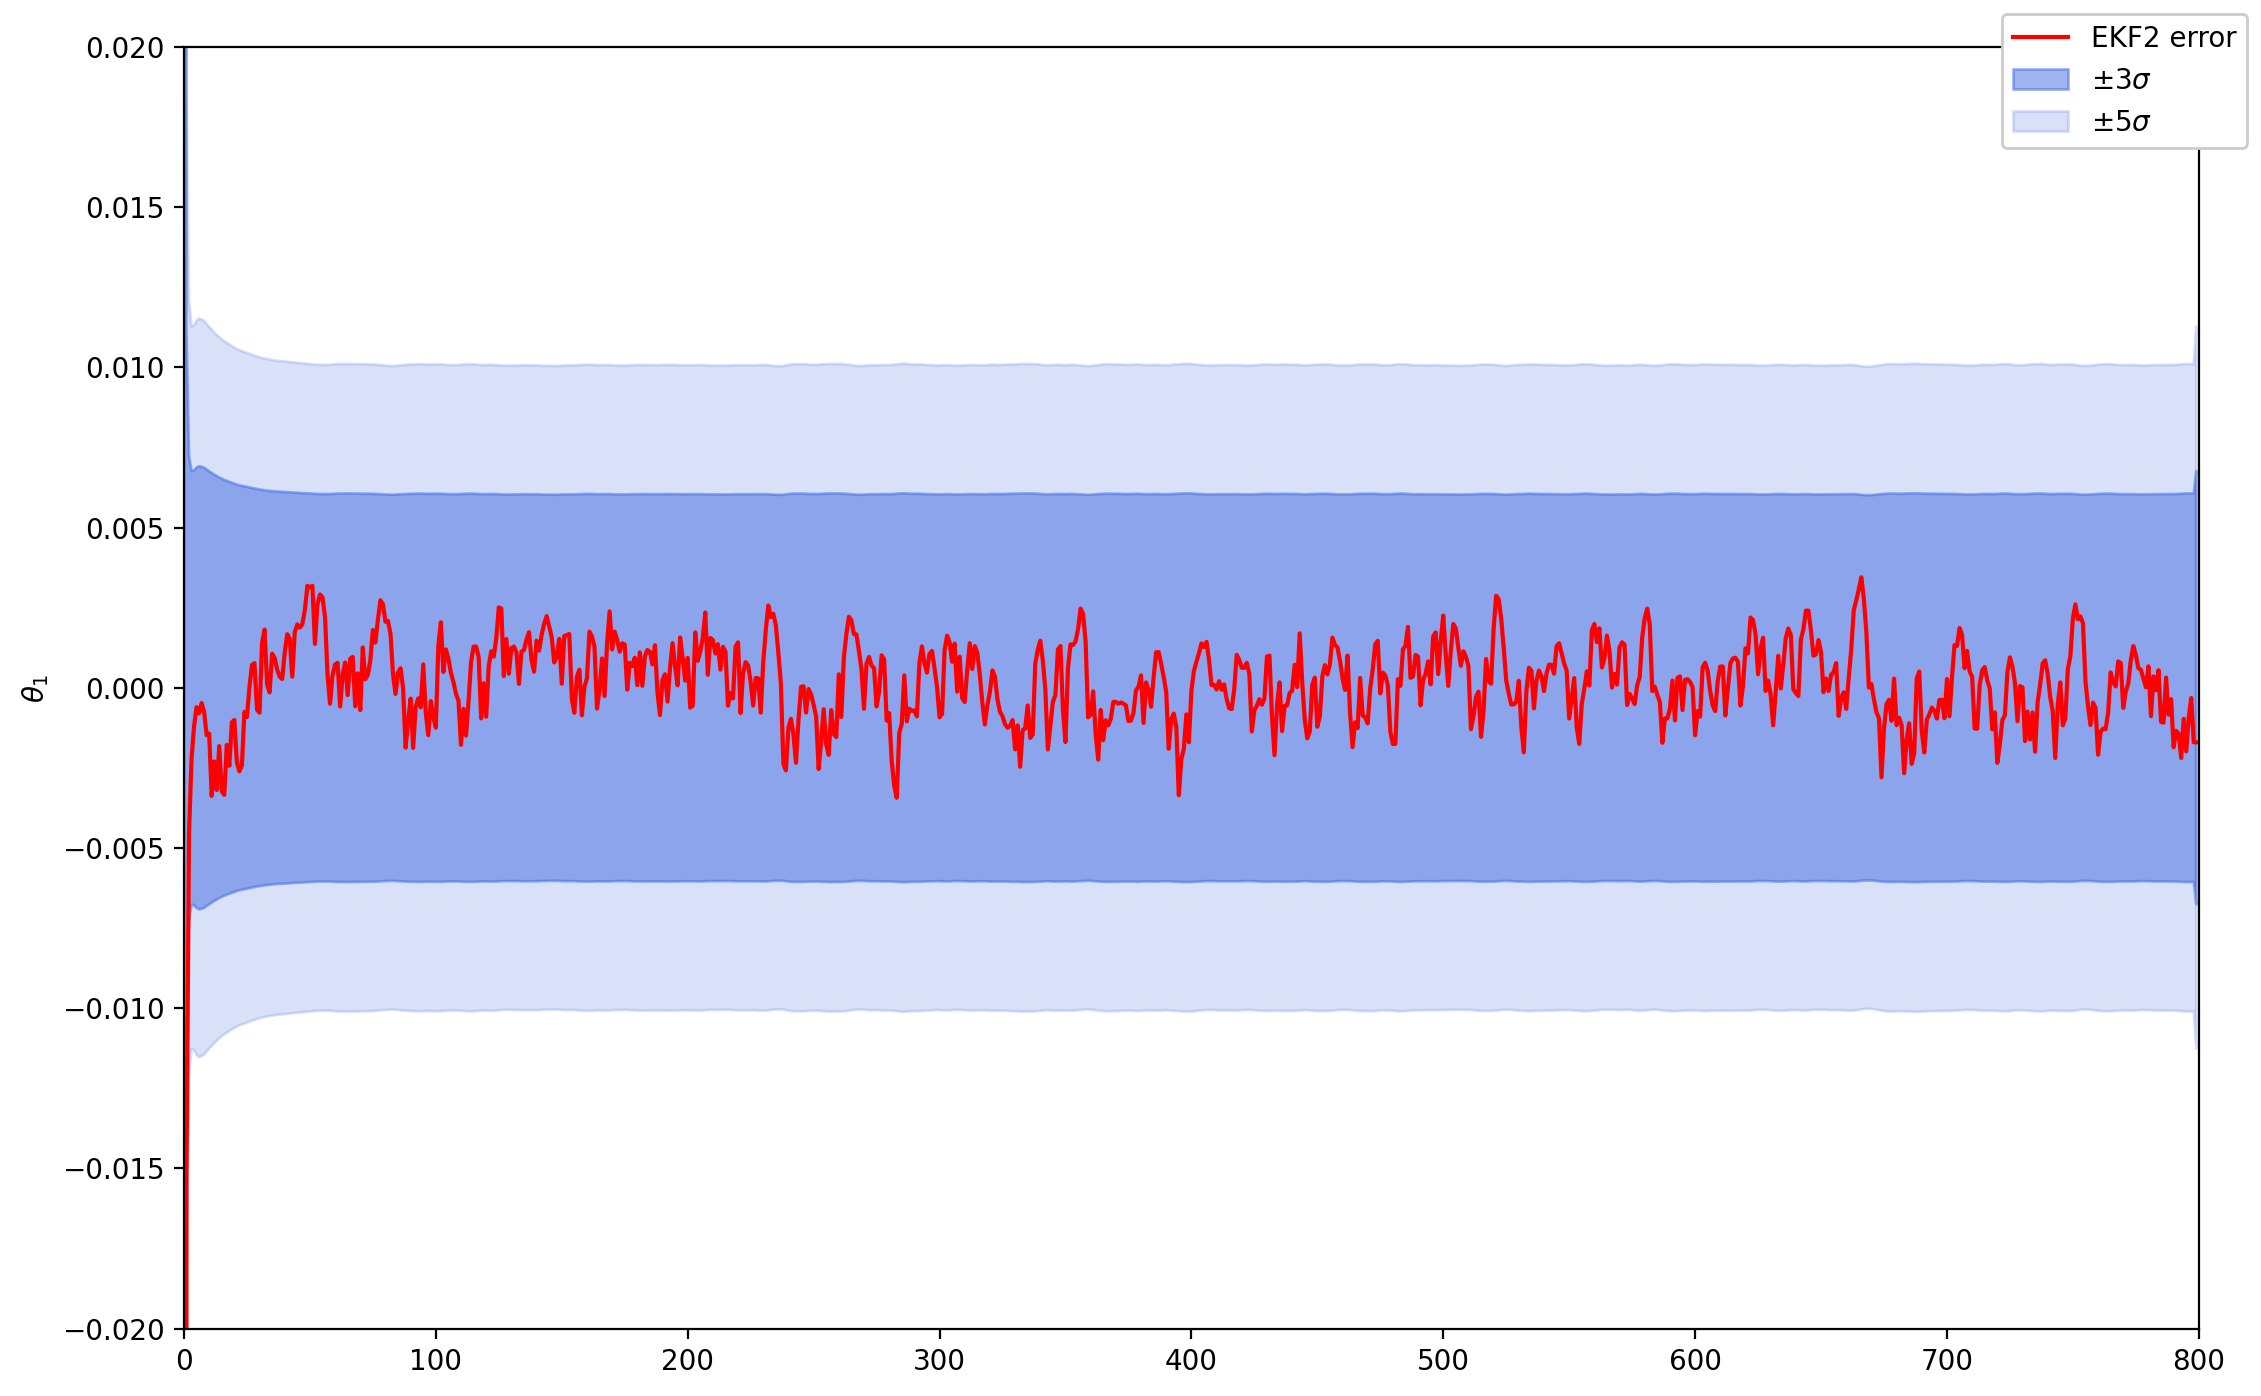
\includegraphics[width=0.95\linewidth]{EKF2_err_theta1.png}
\end{figure}

\begin{figure}[p]
\centering
\caption{EKF2 $\pm 3\sigma(\theta_2)$}
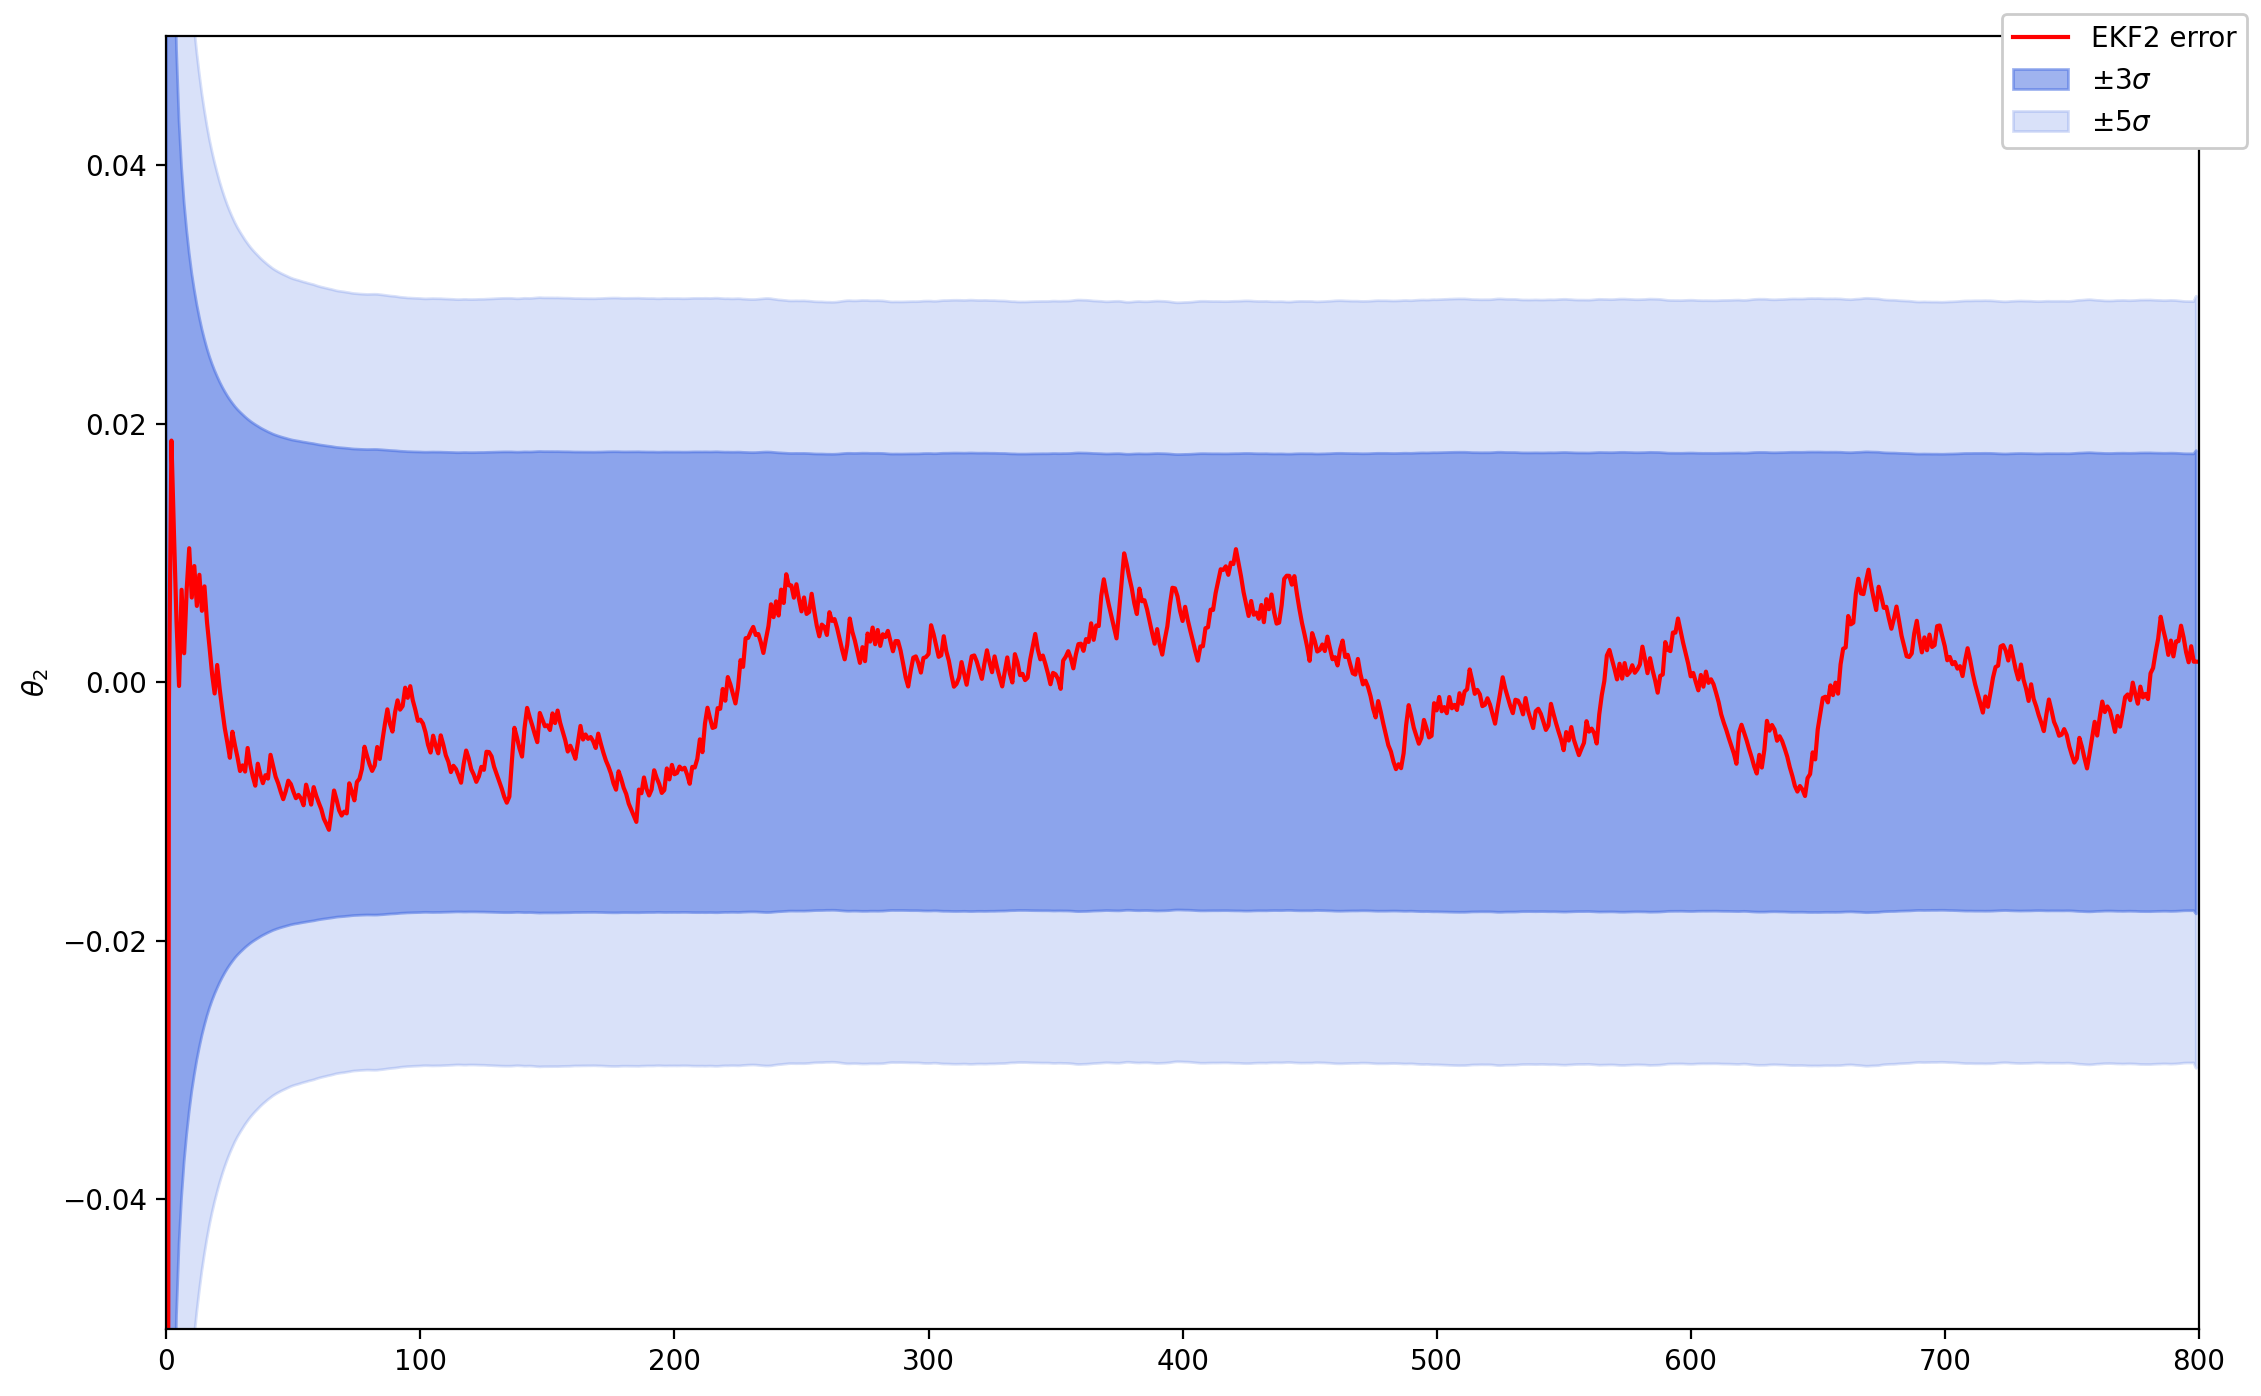
\includegraphics[width=0.95\linewidth]{EKF2_err_theta2.png}
\end{figure}

\begin{figure}[p]
\centering
\caption{SREKF2 $\pm 3\sigma(x_1)$}
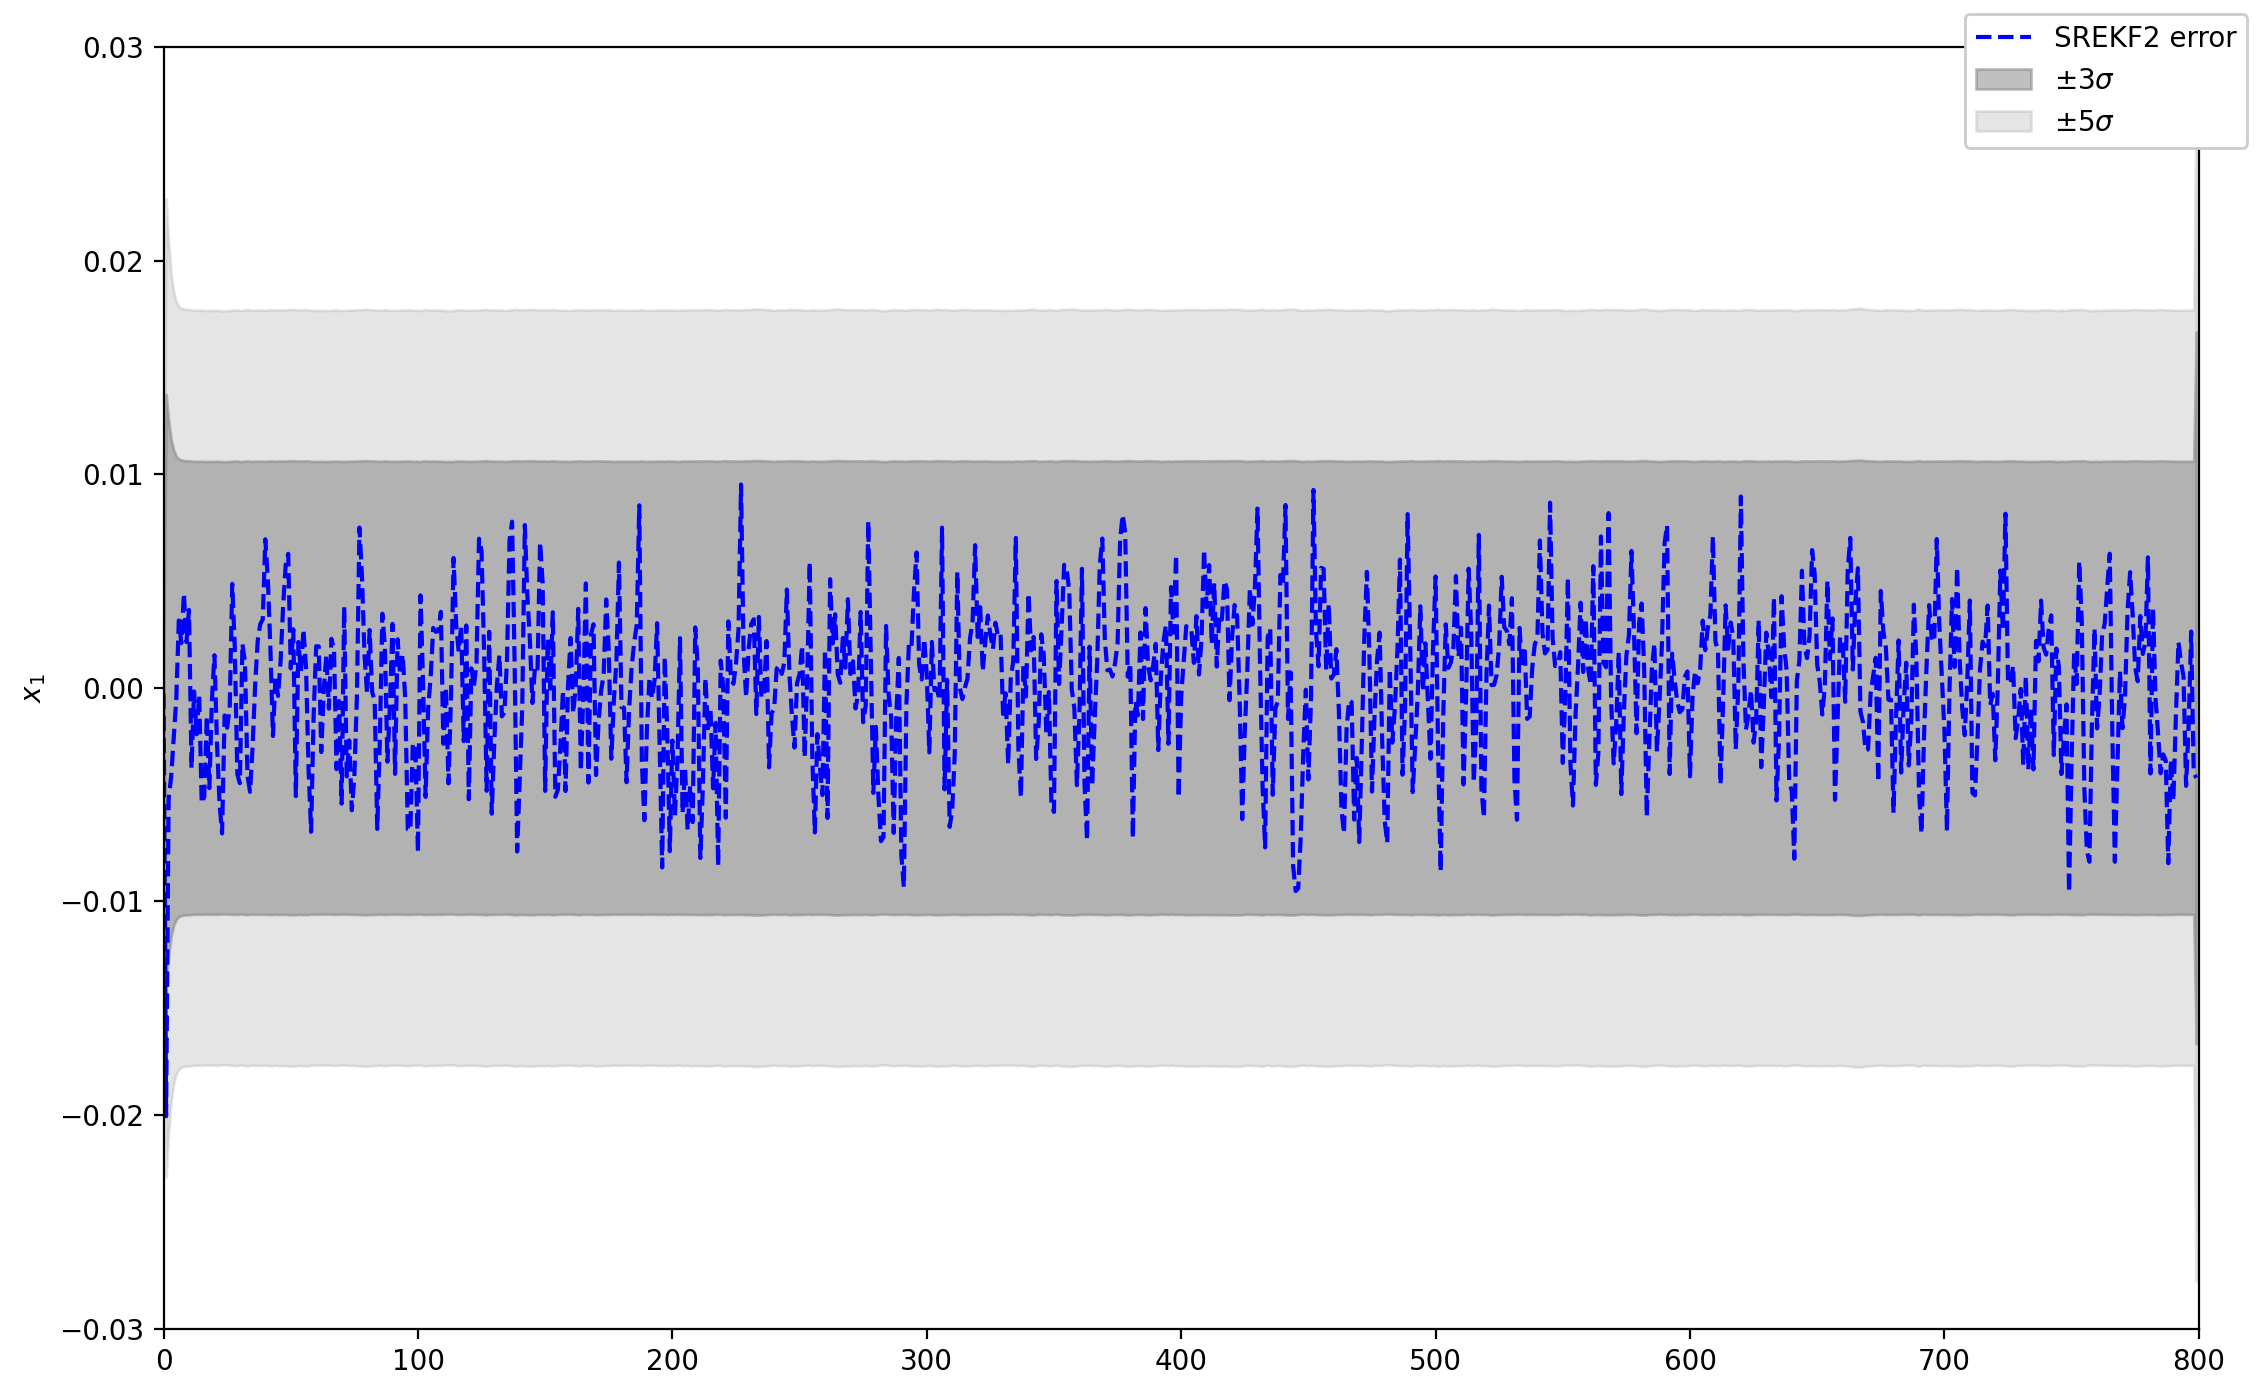
\includegraphics[width=0.95\linewidth]{SREKF2_err_x1.png}
\end{figure}

\begin{figure}[p]
\centering
\caption{SREKF2 $\pm 3\sigma(x_2)$}
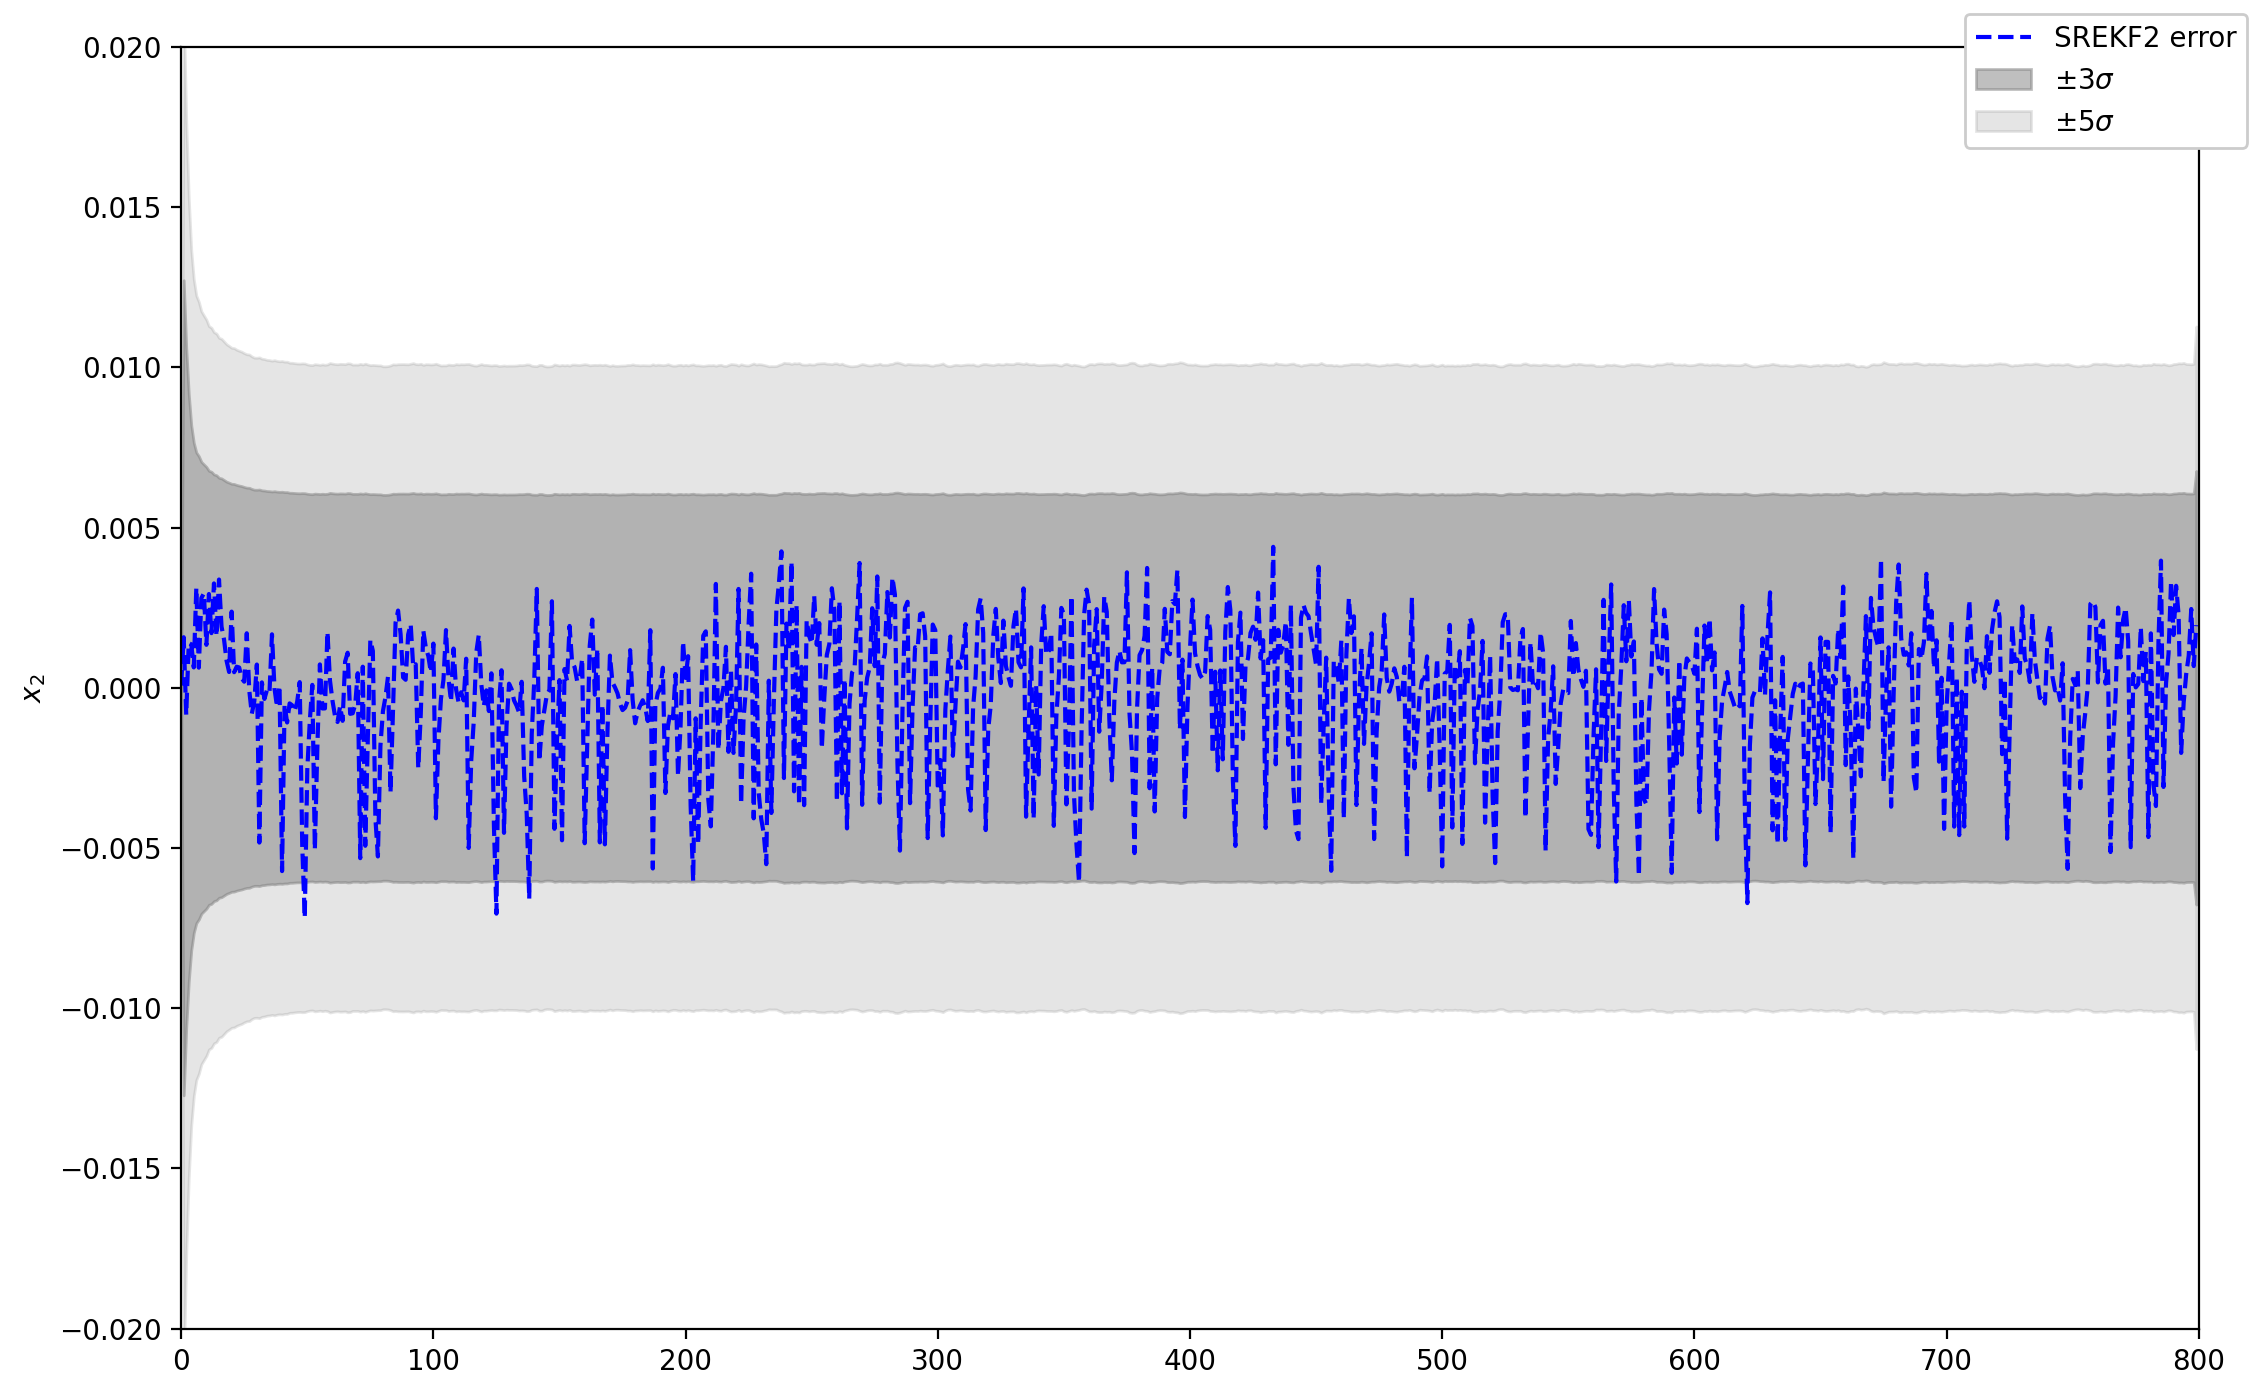
\includegraphics[width=0.95\linewidth]{SREKF2_err_x2.png}
\end{figure}

\begin{figure}[p]
\centering
\caption{SREKF2 $\pm 3\sigma(\theta_1)$}
\includegraphics[width=0.95\linewidth]{SREKF2_err_theta1.png}
\end{figure}

\begin{figure}[p]
\centering
\caption{SREKF2 $\pm 3\sigma(\theta_2)$}
\includegraphics[width=0.95\linewidth]{SREKF2_err_theta2.png}
\end{figure}

\begin{figure}[p]
\centering
\caption{PF $\pm 3\sigma(x_1)$}
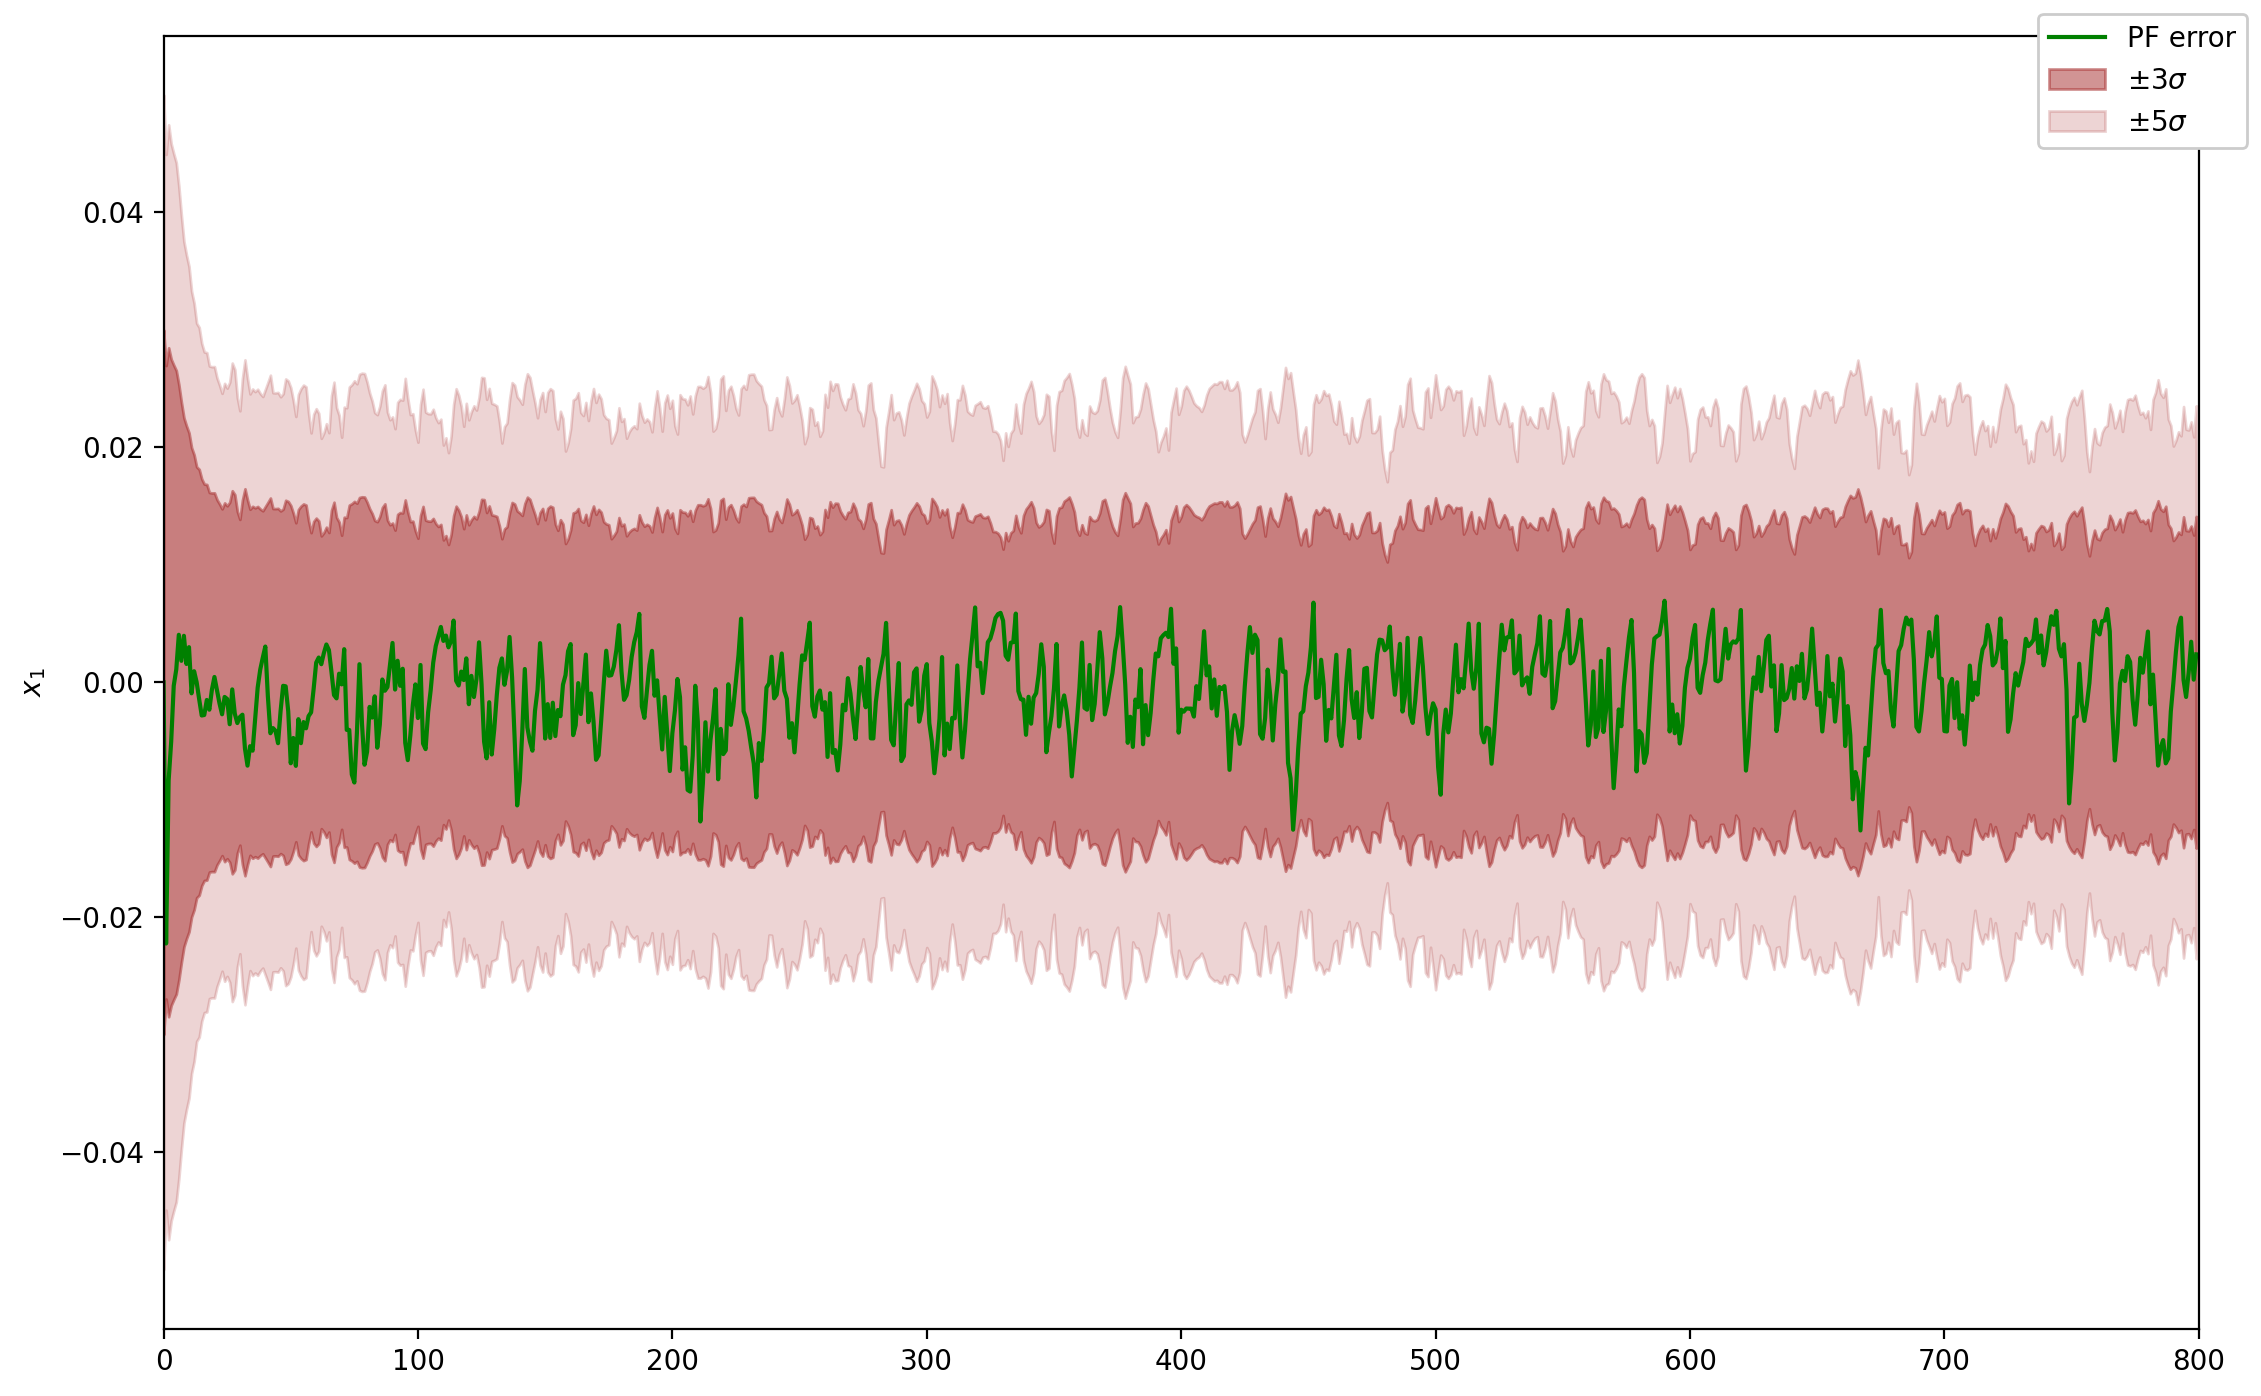
\includegraphics[width=0.95\linewidth]{PF_err_x1.png}
\end{figure}

\begin{figure}[p]
\centering
\caption{PF $\pm 3\sigma(x_2)$}
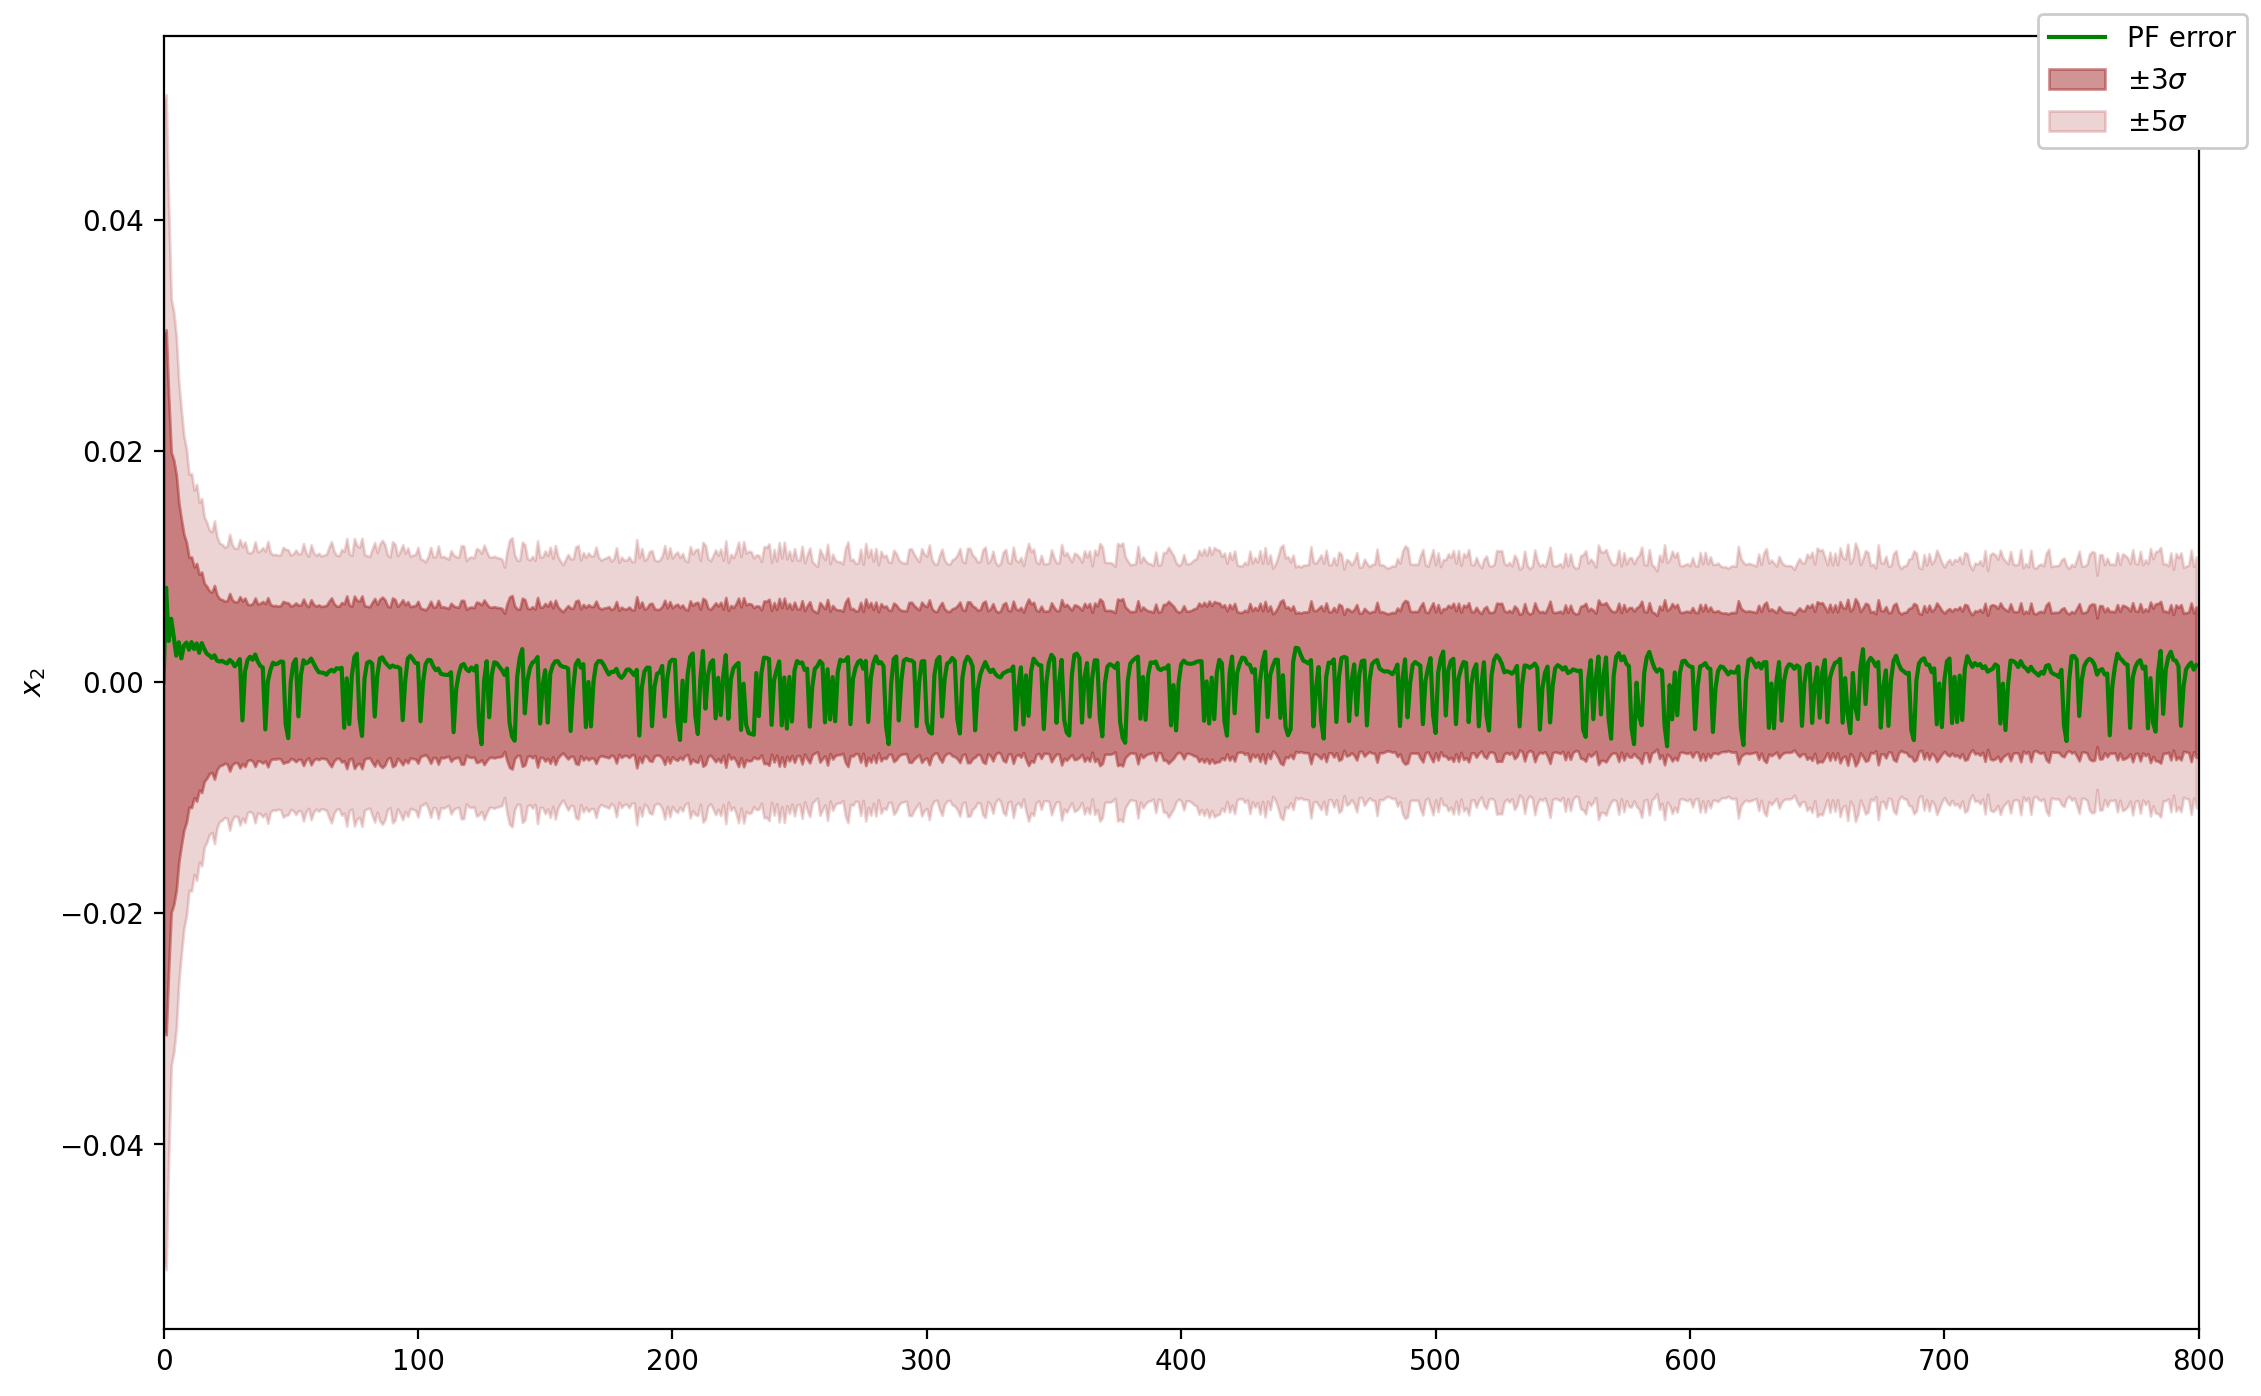
\includegraphics[width=0.95\linewidth]{PF_err_x2.png}
\end{figure}

\begin{figure}[p]
\centering
\caption{PF $\pm 3\sigma(\theta_1)$}
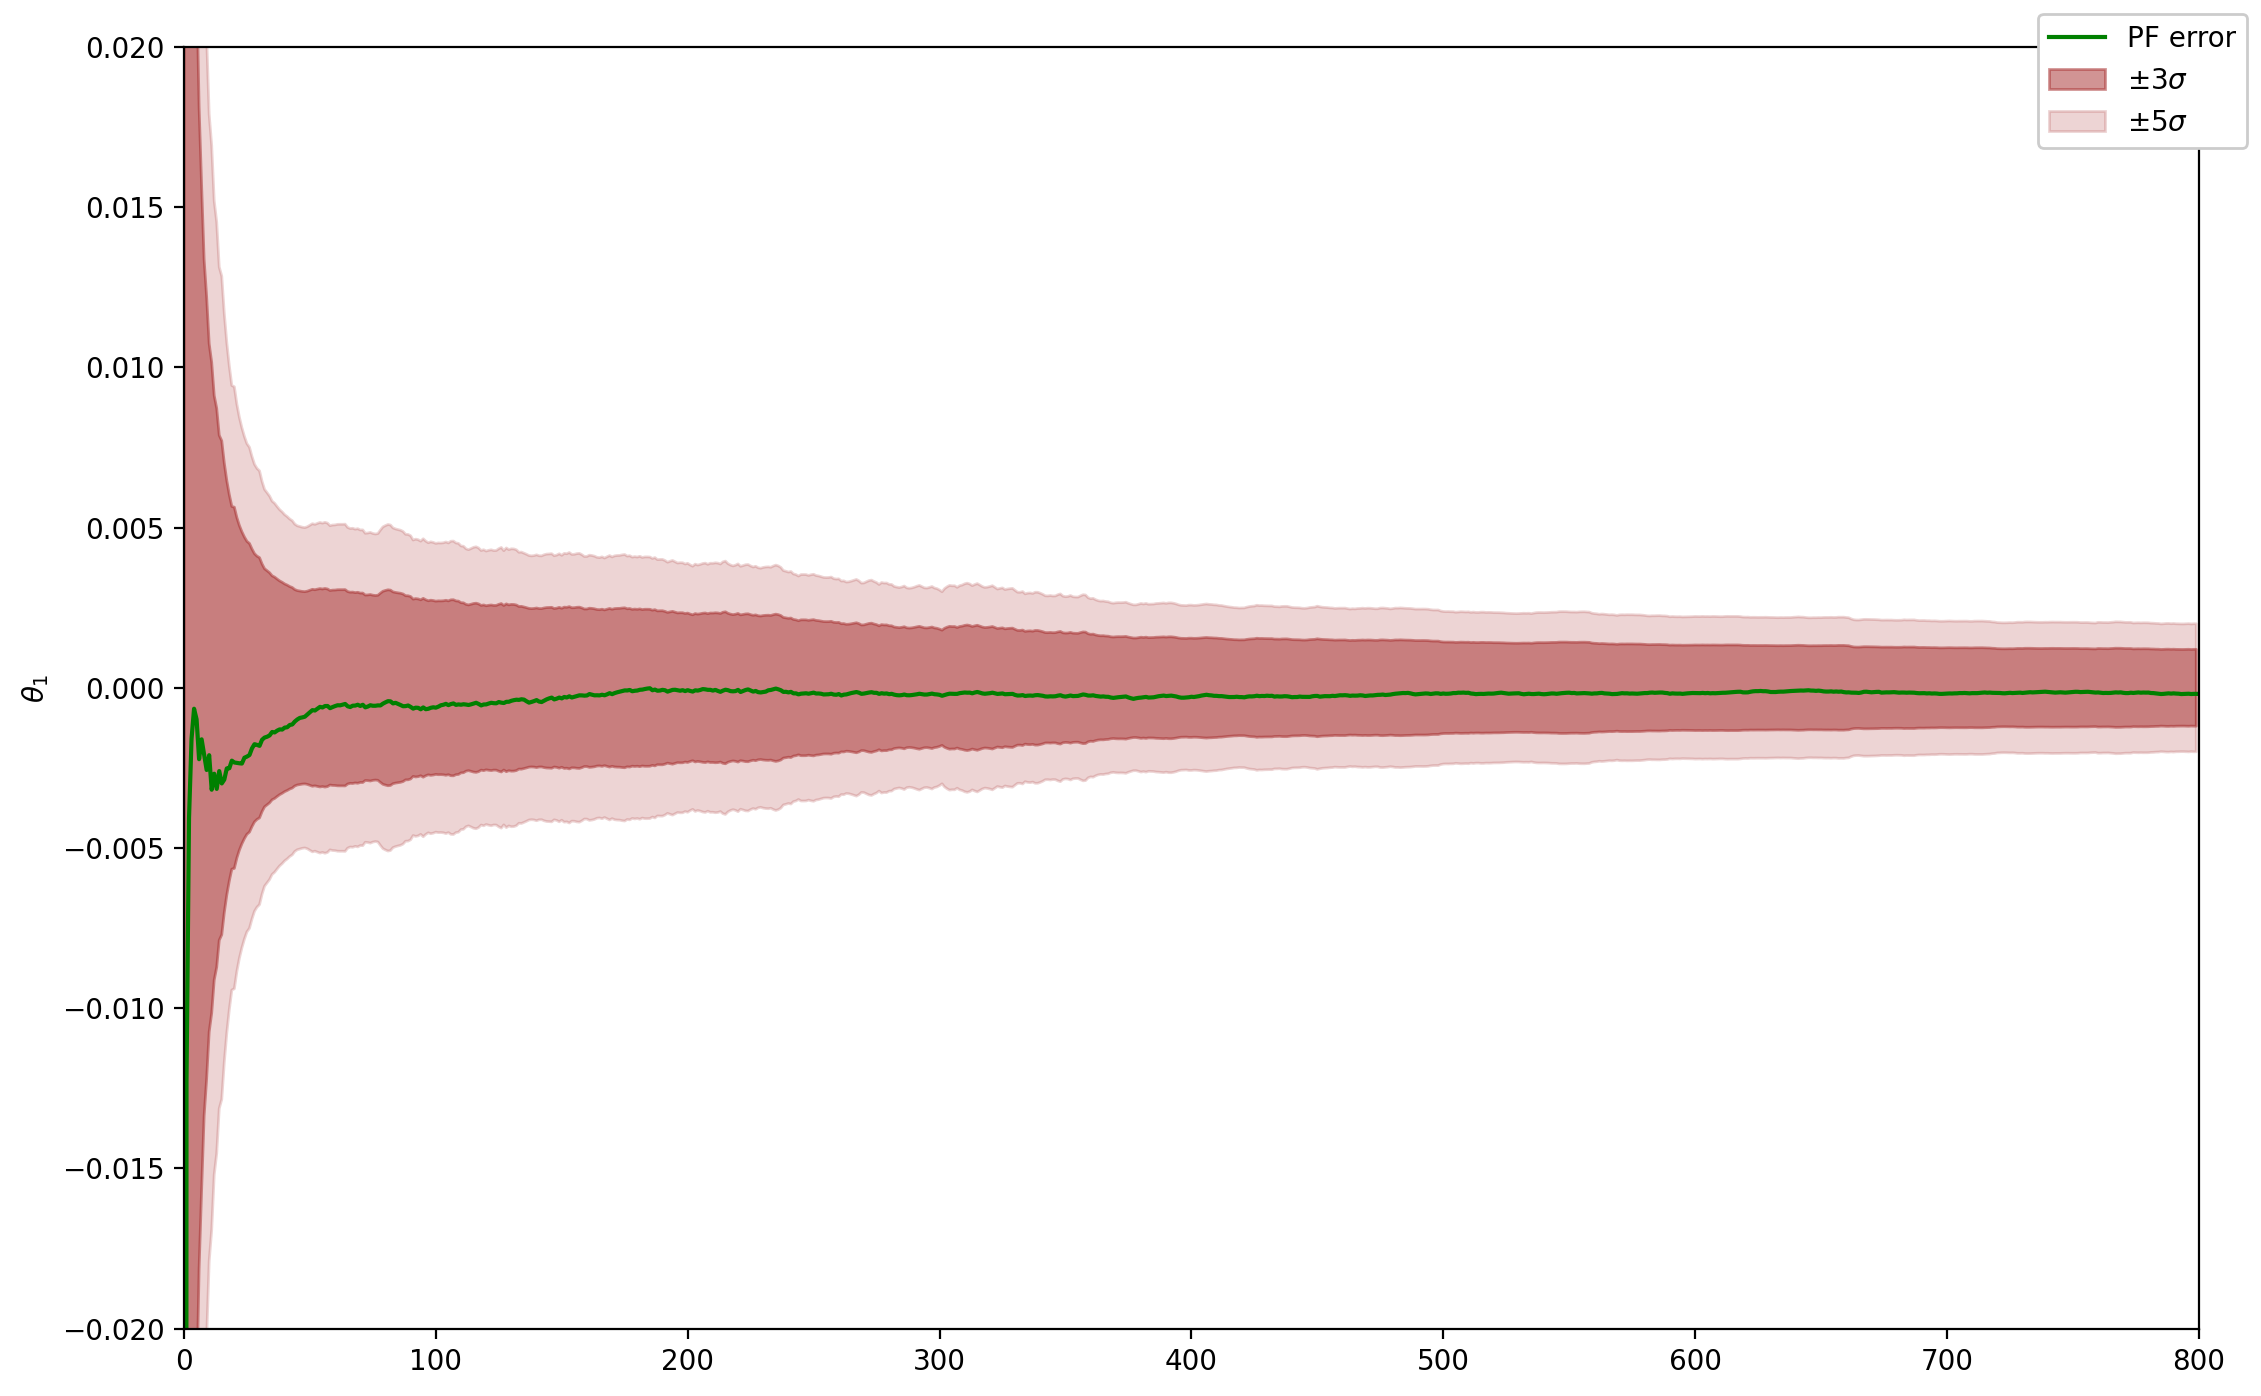
\includegraphics[width=0.95\linewidth]{PF_err_theta1.png}
\end{figure}

\begin{figure}[p]
\centering
\caption{EKF2 $\pm 3\sigma(\theta_2)$}
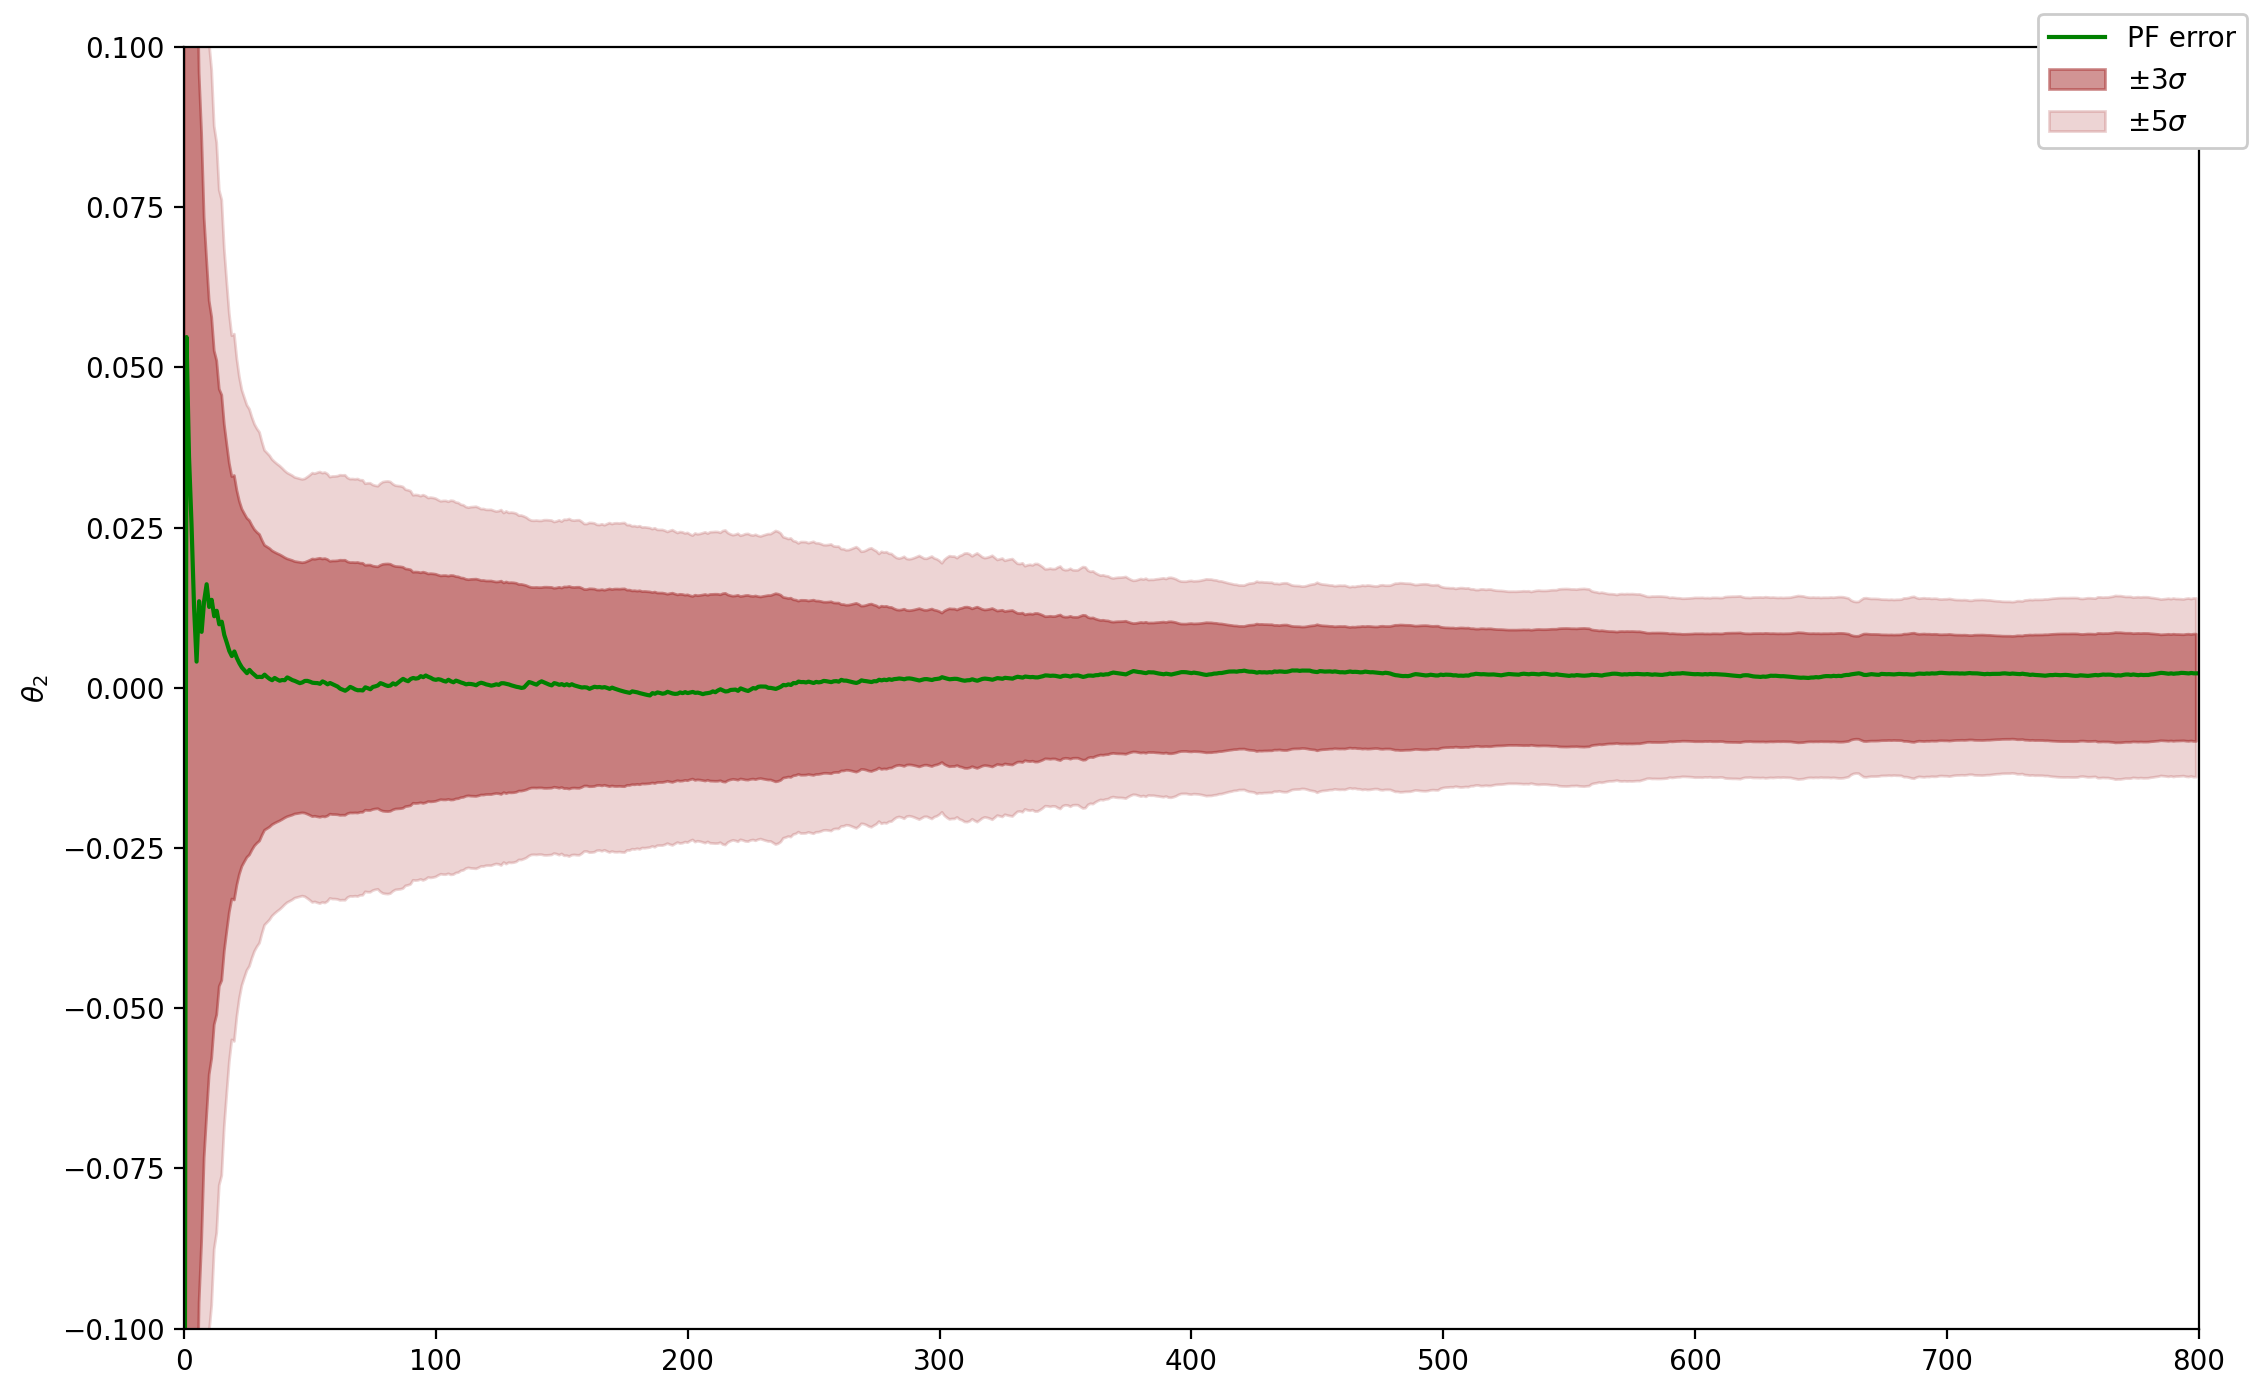
\includegraphics[width=0.95\linewidth]{PF_err_theta2.png}
\end{figure}
\end{landscape}

\subsection{Выборочное СКО ошибок оценивания}

Оценка СКО производилась по выборке объёмом $10000$.

Ниже представлена таблица значений посчитанных СКО в некоторых временных точках и проценты расходящихся траекторий.

\begin{table}[h!]
    \centering
    \begin{tabular}{|c|ccc|}
        \hline
        k &  150 & 400 & 750\\
         \hline
        PF, $x_1$ & 0.00781 & 0.00859 & 0.00922\\
        EKF2, $x_1$ & 0.00377 & 0.00381 & 0.00376\\
        SREKF2, $x_1$ & 0.00376 & 0.0038 & 0.00376\\
        \hline
        PF, $x_2$ &  0.00454 & 0.00545 & 0.00656\\
        EKF2, $x_2$ & 0.00224 & 0.00229 & 0.00228\\
        SREKF2, $x_2$ & 0.00224 & 0.00231 & 0.00229\\
        \hline
        PF, $\theta_1$ & 0.00402 & 0.005 & 0.00616\\
        EKF2, $\theta_1$ & 0.00123 & 0.00123 & 0.00124\\
        SREKF2, $\theta_1$ & 0.00124 & 0.0013 & 0.00135\\
        \hline
        PF, $\theta_2$ & 0.02845 & 0.03416 & 0.04164\\
        EKF2, $\theta_2$ & 0.00417 & 0.00411 & 0.00419\\
        SREKF2, $\theta_2$ & 0.00417 & 0.00412 & 0.0042 \\
        \hline
    \end{tabular}
    \caption{Значения СКО в некоторых точках}
    \label{tab:emse}
\end{table}

\begin{table}[h!]
    \centering
    \begin{tabular}{|c|c|c|}
        \hline
        EKF2      & SREKF2    & PF \\
        \hline
        $0.02 \%$ & $0.02 \%$ & $57.58 \%$ \\
        \hline
    \end{tabular}
    \caption{Проценты расходящихся траекторий}
    \label{tab:divergence_percentage}
\end{table}

Далее представлены графики полученных оценок.

\begin{landscape}
\begin{figure}[p]
\centering
\caption{Сравнение СКО ошибок оценок $x_1$}
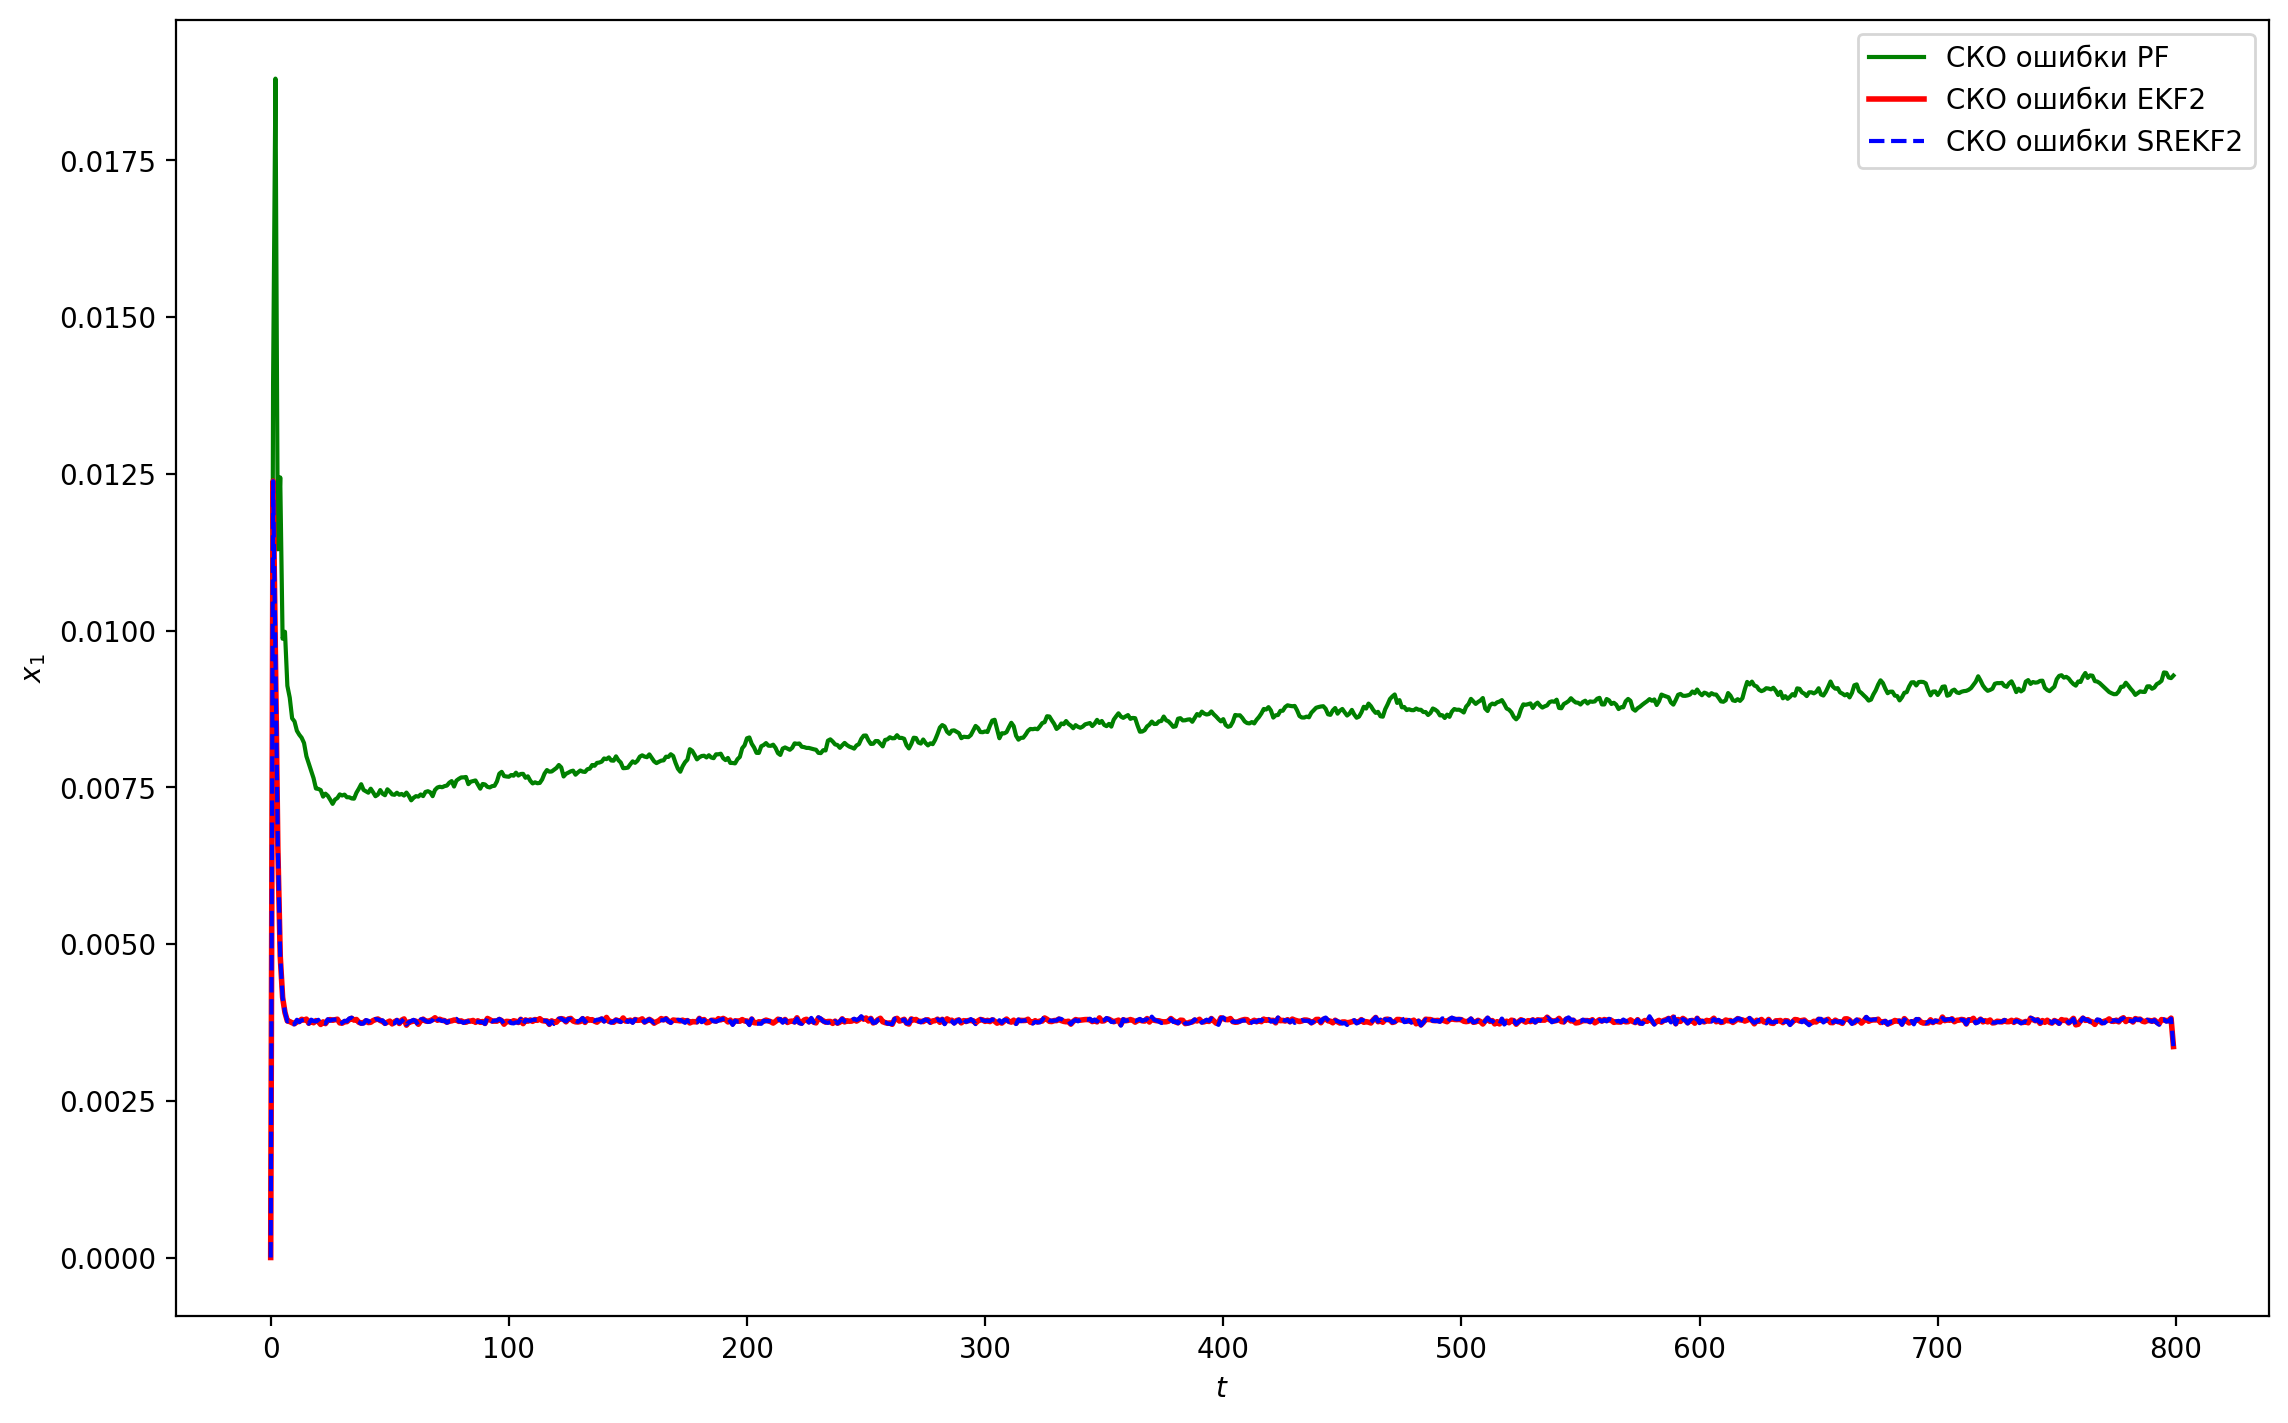
\includegraphics[width=0.95\linewidth]{RMSE_x1.png}

\end{figure}

\begin{figure}[p]
\centering
\caption{Сравнение СКО ошибок оценок $x_2$}
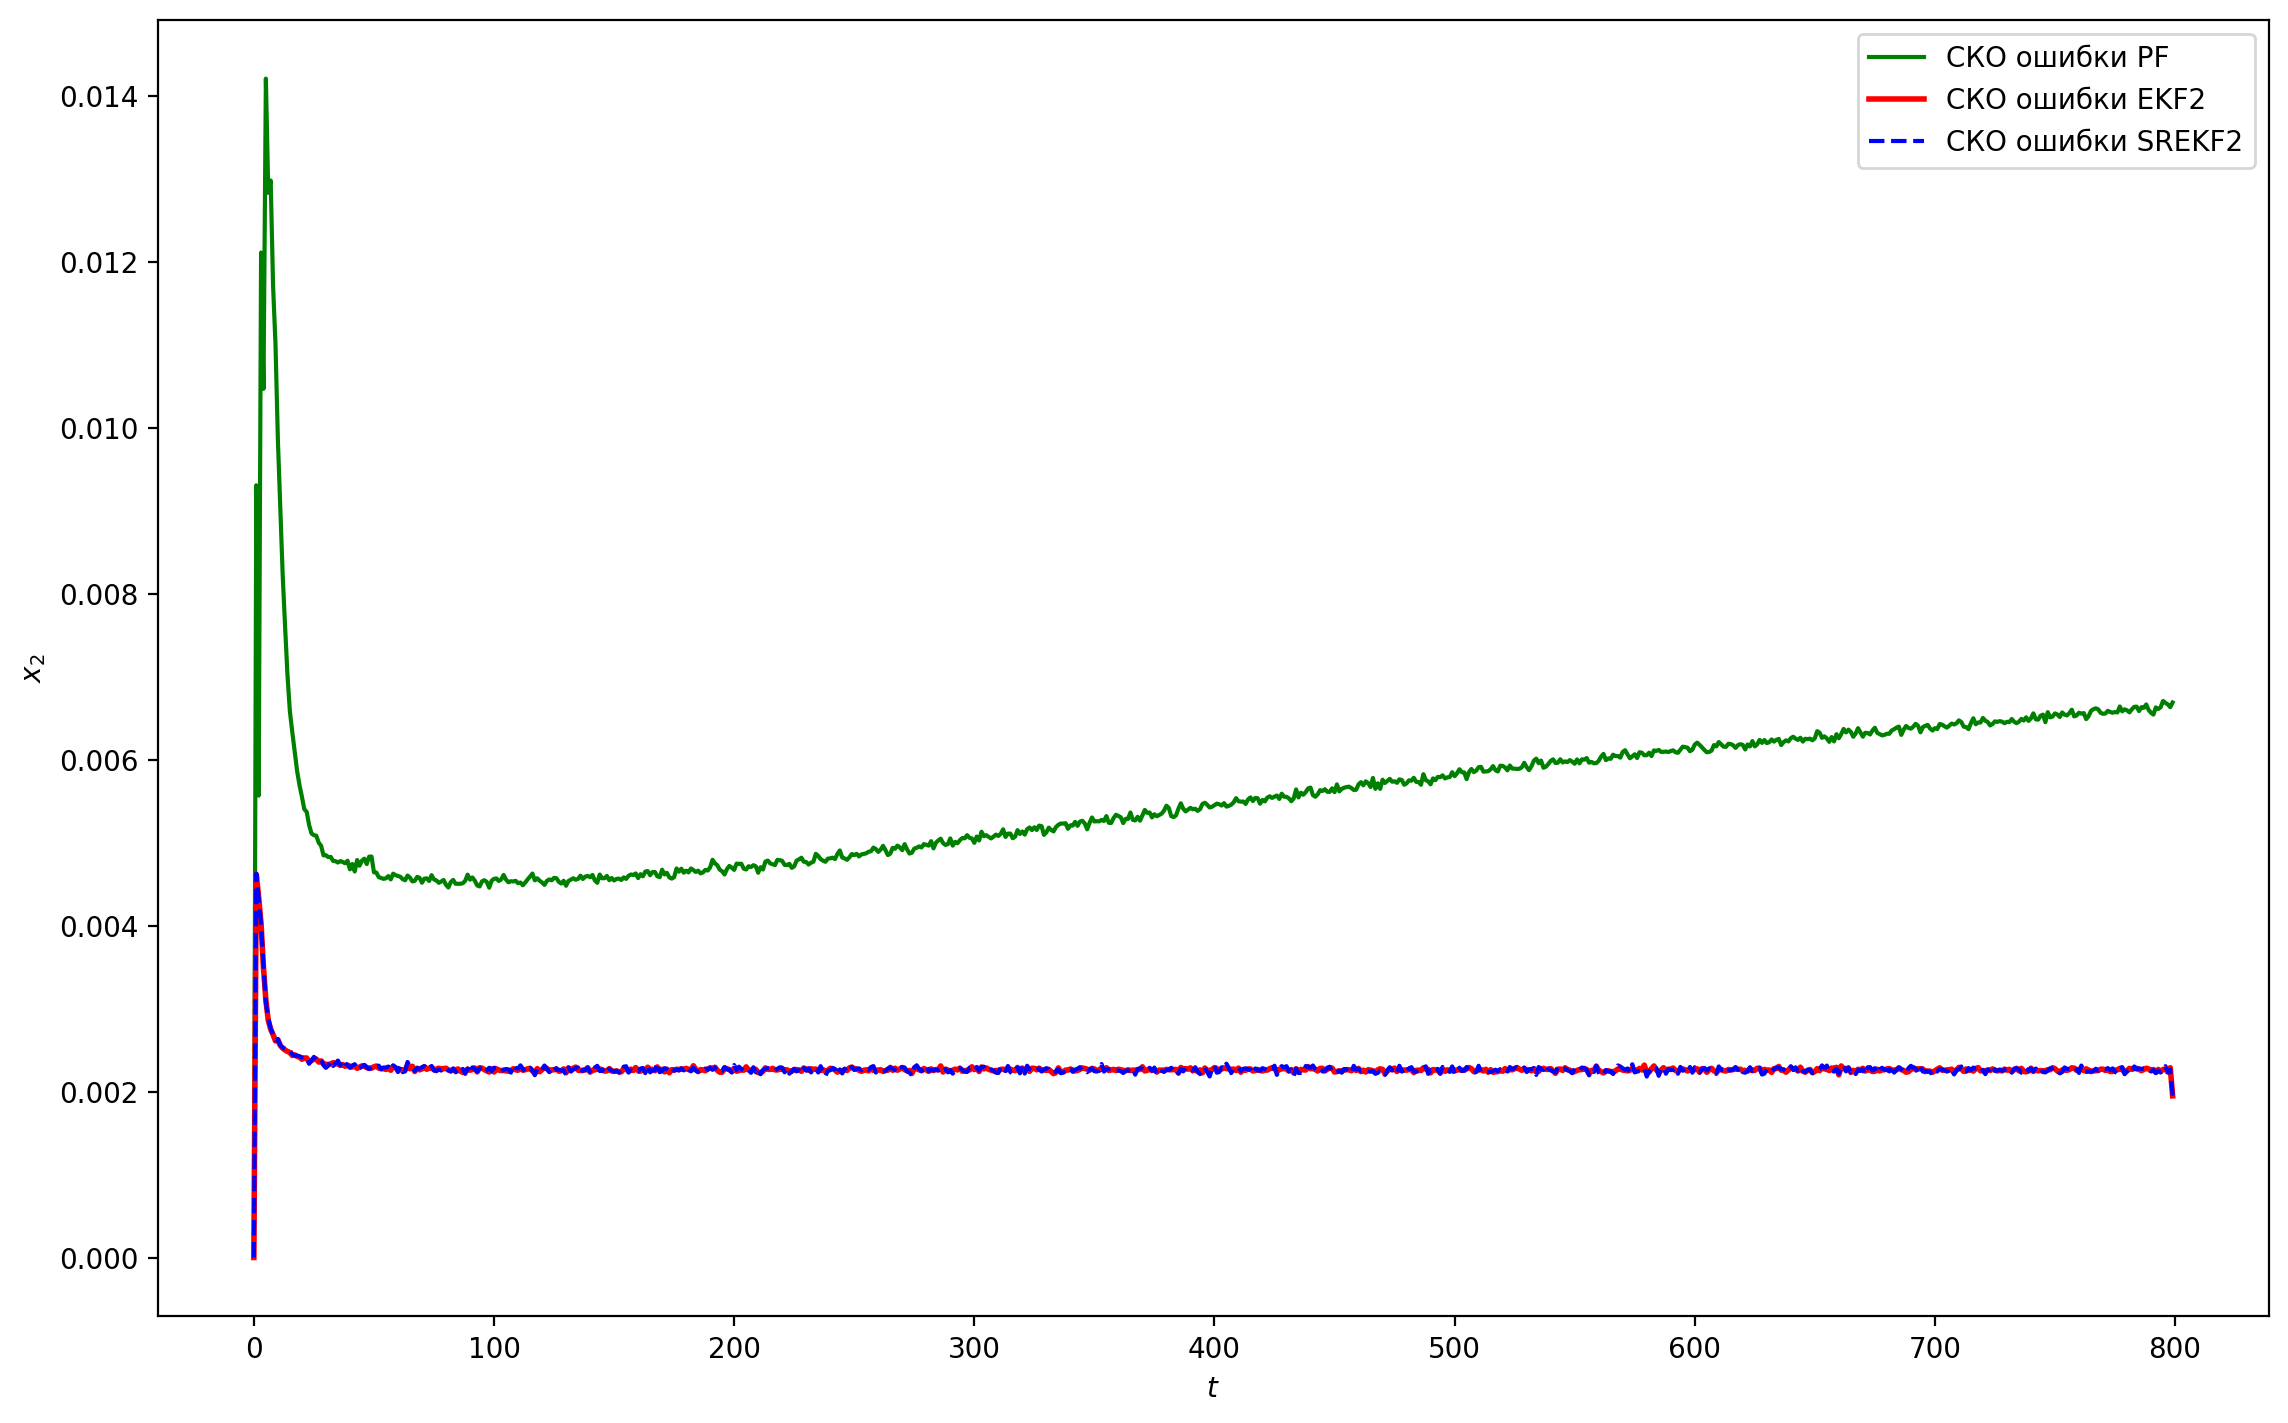
\includegraphics[width=0.95\linewidth]{RMSE_x2.png}

\end{figure}

\begin{figure}[p]
\centering
\caption{Сравнение СКО ошибок оценок $\theta_1$}
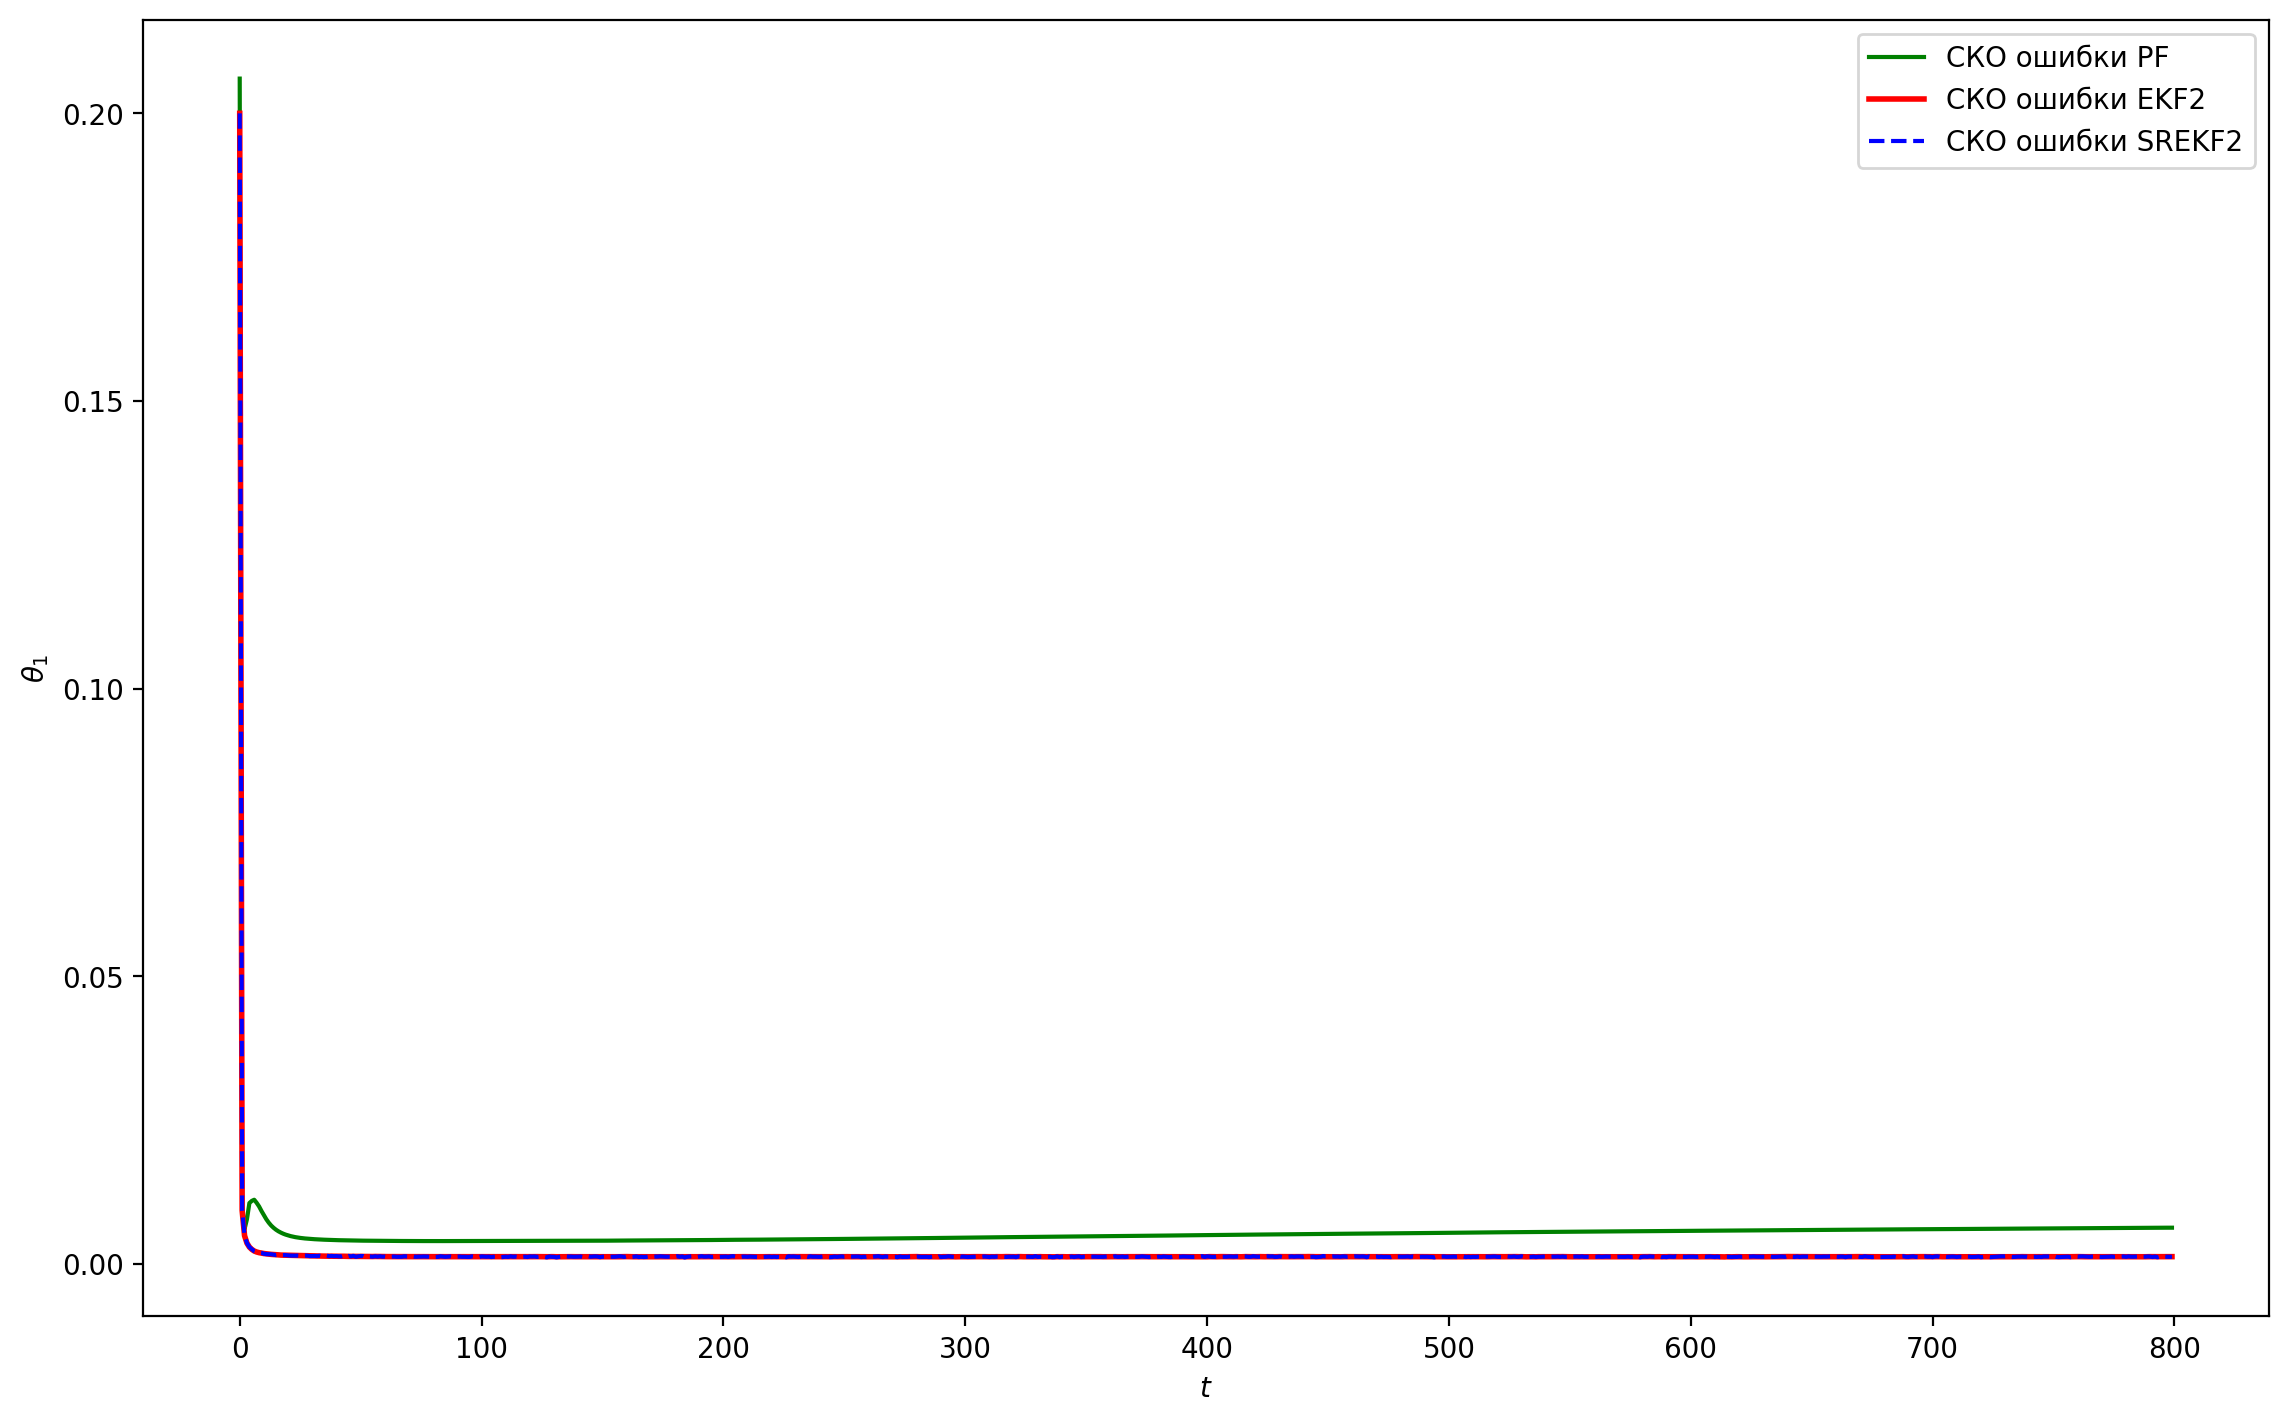
\includegraphics[width=0.95\linewidth]{RMSE_theta1.png}

\end{figure}

\begin{figure}[p]
\centering
\caption{Сравнение СКО ошибок оценок $\theta_2$}
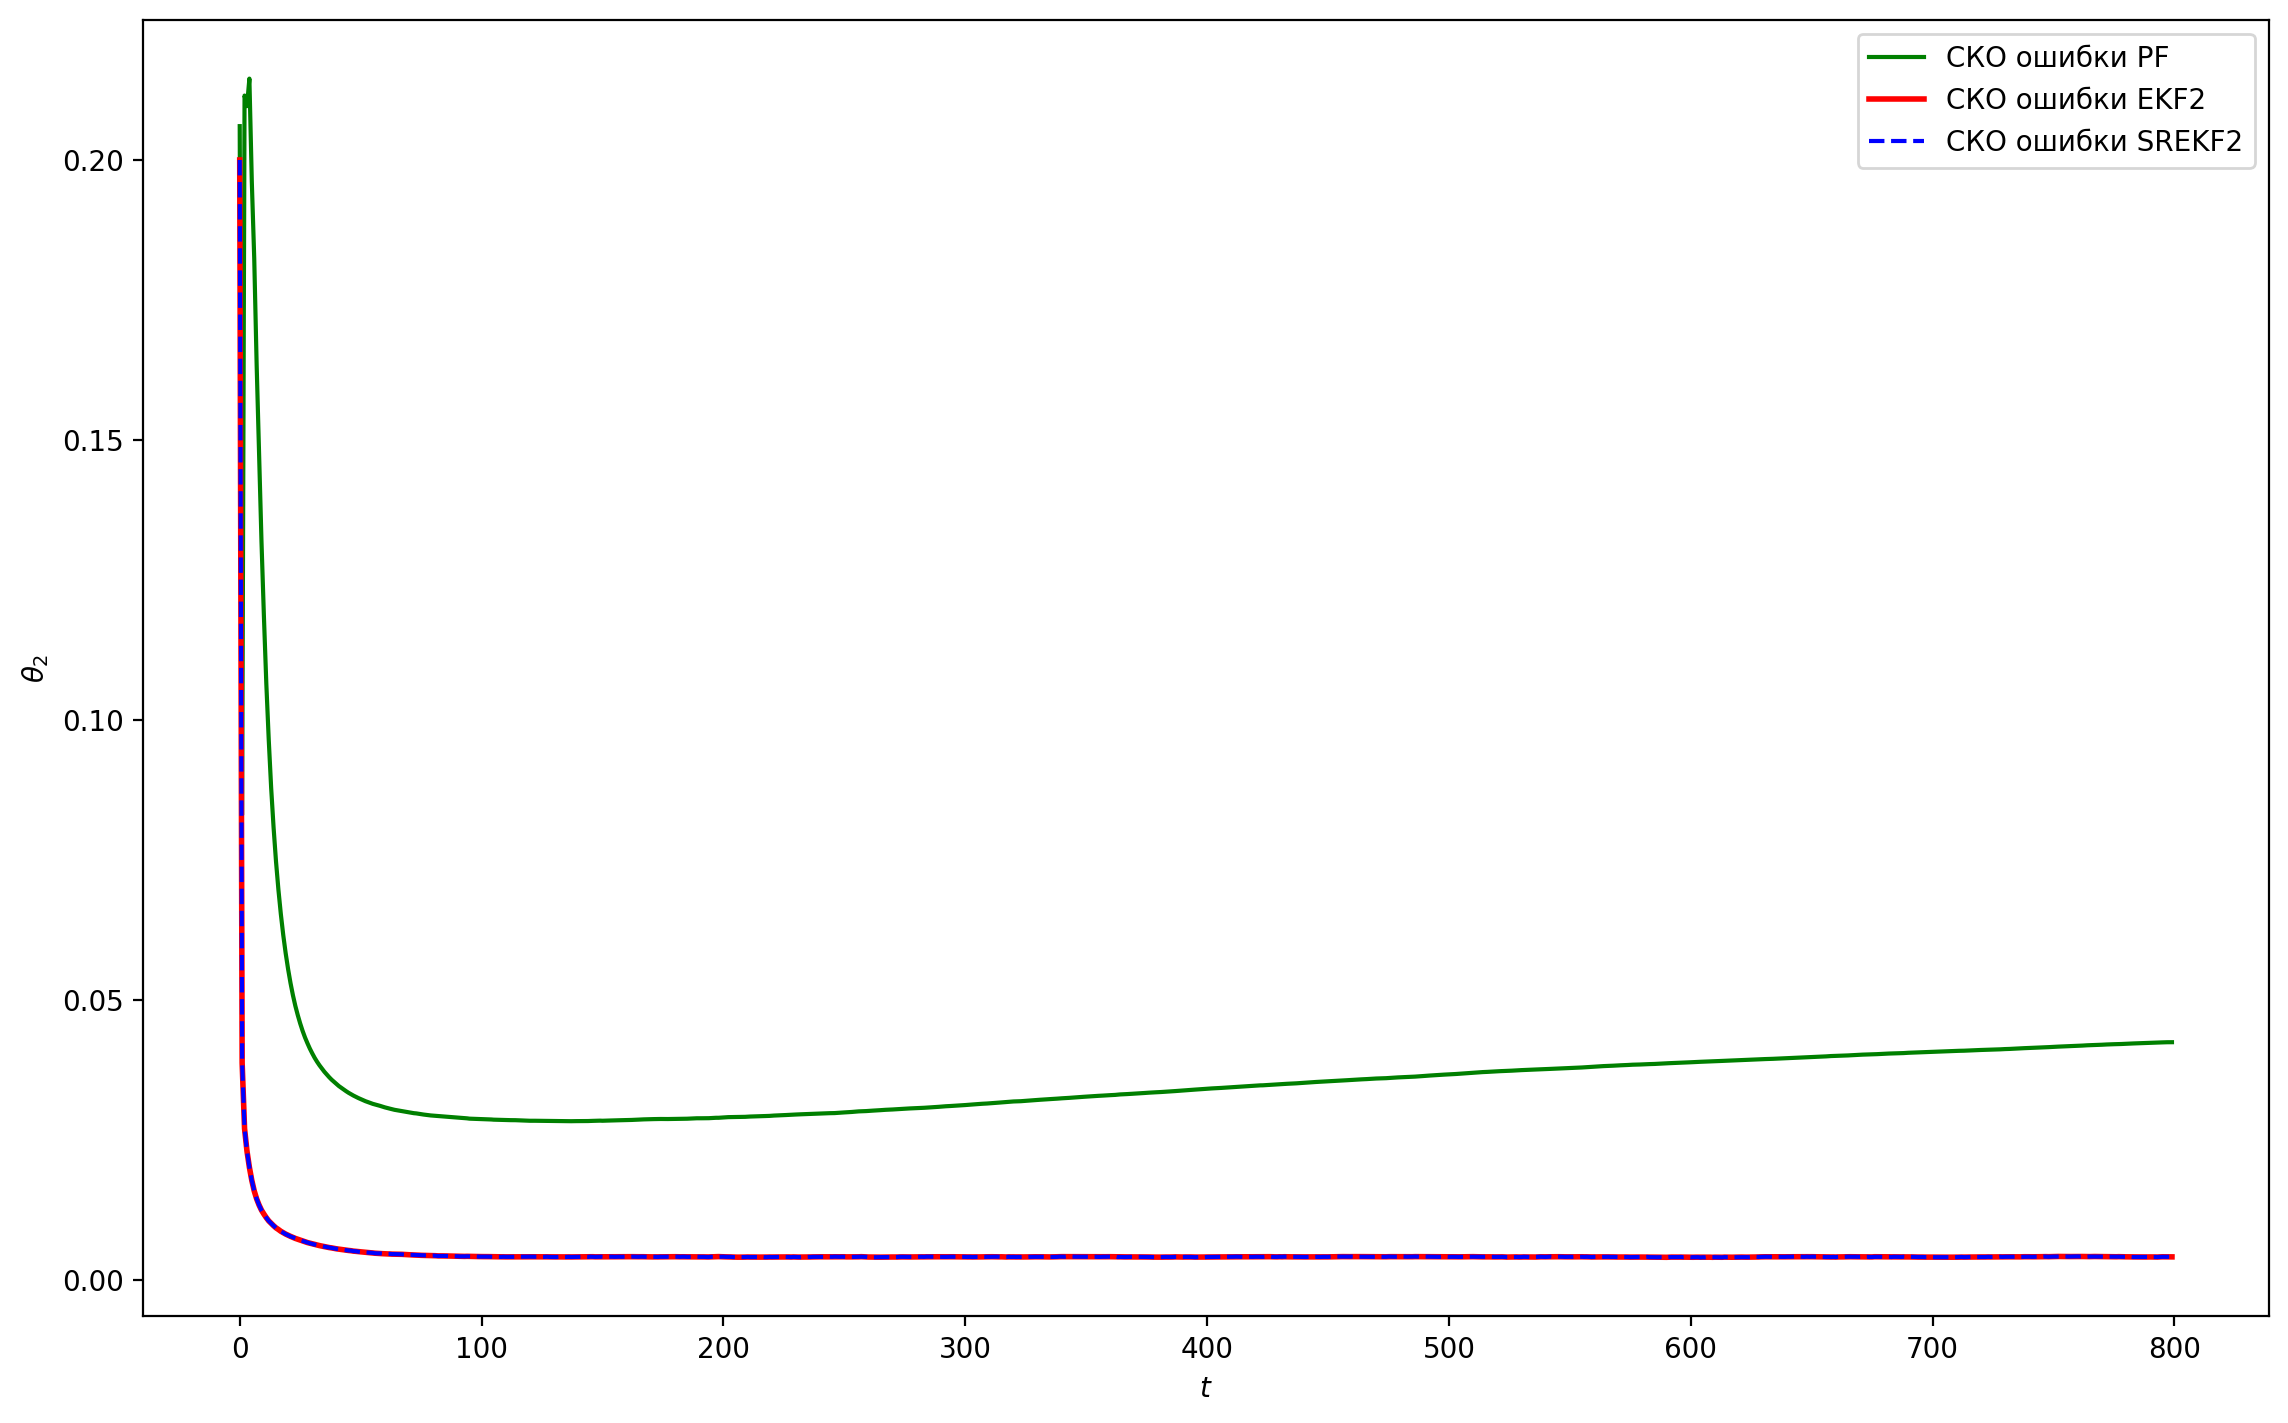
\includegraphics[width=0.95\linewidth]{RMSE_theta2.png}
\end{figure}
\end{landscape}

\section{Выводы}

Для данной системы оценки расширенного фильтра Калмана и его корневого варианты оказались идентичными по качеству. Следовательно, для данной задачи предпочтительным является EKF2, так как требует меньше арифметических операций. 

В то же время, бутстреп фильтр уступает и по точности оценивания, и по количеству расходящихся траекторий. Данные проблемы можно объяснить нестандартными шумами в системе.

Расширенный фильтр Калмана оказался наиболее подходящим для данной задачи, демонстрируя крайне маленьких процент расходимости и высокое качество. 

\end{document}
